\documentclass[11pt]{article}
\usepackage[T1]{fontenc}
\usepackage{lmodern}
\input{glyphtounicode-cmex}
\usepackage{amsmath,amssymb,amsthm,mathtools}
\usepackage[margin=1in]{geometry}
\usepackage{microtype}
\usepackage{enumitem}
\usepackage{placeins}
\usepackage{tikz}
\usetikzlibrary{arrows.meta,positioning}
\usepackage[hidelinks]{hyperref}
\hypersetup{pdftitle={Relative independence of the separable quotient problem},pdfauthor={OpenAI}}
\newtheorem{theorem}{Theorem}[section]
\newtheorem{lemma}[theorem]{Lemma}
\newtheorem{proposition}[theorem]{Proposition}
\newtheorem{corollary}[theorem]{Corollary}
\theoremstyle{definition}
\newtheorem{definition}[theorem]{Definition}
\newtheorem{remark}[theorem]{Remark}
\newcommand{\R}{\mathbb R}
\newcommand{\C}{\mathbb C}
\newcommand{\N}{\mathbb N}
\newcommand{\Q}{\mathbb Q}
\DeclareMathOperator{\dist}{dist}
\DeclareMathOperator{\supp}{supp}
\DeclareMathOperator{\dens}{dens}
\DeclareMathOperator{\ran}{ran}
\DeclareMathOperator{\absconv}{absconv}
\newcommand{\clspan}[1]{\overline{\operatorname{span}}\{#1\}}
\newcommand{\SQ}{\mathrm{SQ}}
\setlength{\emergencystretch}{2em}
\title{Relative independence of the separable quotient problem}
\author{OpenAI}
\date{September 23, 2026}
\begin{document}
\maketitle
\begin{abstract}
The separable quotient problem asks whether every infinite-dimensional Banach
space has a separable infinite-dimensional quotient. We prove that this
statement is independent of ZFC, relative to the consistency of ZFC with a
measurable cardinal. This holds over both the real and complex fields. For
spaces of norm density $\aleph_1$, we obtain independence relative to the
consistency of ZFC alone.
\end{abstract}
\setcounter{tocdepth}{1}
\tableofcontents
\clearpage
\section{Introduction}\label{sec:introduction}

Every infinite-dimensional Banach space contains a separable
infinite-dimensional closed subspace: take the closed span of a countable
linearly independent set. The corresponding assertion for quotients is the
\emph{separable quotient problem}, traditionally attributed to Banach and
Mazur. For a scalar field $\mathbb F\in\{\R,\C\}$, let $\SQ_{\mathbb F}$
denote the statement
\begin{quote}
Every infinite-dimensional Banach space over $\mathbb F$ admits a
bounded linear surjection onto a separable infinite-dimensional
Banach space.
\end{quote}
Equivalently, each such space $X$ has a closed subspace $M$ for which
$X/M$ is separable and infinite dimensional. The equivalence follows by
applying the open mapping theorem to the induced bijection from a space
modulo the kernel of a surjection.

We work with the axiom of Choice throughout. Write
$\mathfrak c=2^{\aleph_0}$ for the cardinality of the continuum.
For an uncountable cardinal $\kappa$, a probability measure on
$\mathcal P(\kappa)$ is \emph{$\kappa$-additive} if it is additive on
pairwise disjoint families of cardinality strictly less than $\kappa$;
the sum over such a family means the supremum of its finite subsums.
We say that $\kappa$ is \emph{real-valued measurable} if it carries such
a measure vanishing on singletons. In particular, the hypothesis below
requires a measure on \emph{every subset} of $\mathfrak c$, with this
stronger additivity property.

The two implications below are proved in ZFC. Their hypotheses are then
realized in models at the indicated consistency strengths; this gives
the relative-independence conclusion.

\begin{theorem}\label{intro:main}
For each $\mathbb F\in\{\R,\C\}$, ZFC proves the following implications.
\begin{enumerate}[label=\textup{(\roman*)}]
 \item If $\mathfrak c$ is real-valued measurable, then $\SQ_{\mathbb F}$
 holds.
 \item If the continuum hypothesis holds, then $\SQ_{\mathbb F}$ fails.
\end{enumerate}
Consequently, if ZFC with a measurable cardinal is consistent, then
$\SQ_{\mathbb F}$ is independent of ZFC. Consistency of its failure
requires only consistency of ZFC.
\end{theorem}

The CH counterexamples already occur at norm density $\aleph_1$, the
smallest possible nonseparable density (Corollary~\ref{twist:density}).
At this density, an earlier positive theorem yields a sharper consistency
conclusion. Let $\SQ^{\aleph_1}_{\mathbb F}$ denote the assertion that
every Banach space over $\mathbb F$ of norm density exactly $\aleph_1$
has a separable infinite-dimensional quotient.

\begin{corollary}\label{intro:small-density}
If ZFC is consistent, then $\SQ^{\aleph_1}_{\mathbb F}$ is independent
of ZFC for each $\mathbb F\in\{\R,\C\}$.
\end{corollary}

The positive side of this corollary uses the density criterion of Saxon
and S\'anchez Ruiz described below, together with Martin's axiom. The
negative side uses the counterexample constructed here. The measurable
cardinal hypothesis in Theorem~\ref{intro:main} concerns the unrestricted
quotient assertion.

\paragraph{History and methods.}
The history and many positive cases of the problem are surveyed
in~\cite{Brech2025,FerrandoKakolLopezPellicerSliwa2018}.
Brech notes that the problem is not stated explicitly in Banach's 1932
book and identifies Rosenthal's 1969 paper as an early written
formulation~\cite[p.~74]{Brech2025}.
Johnson and Rosenthal developed the weak-star basic-sequence method and
proved that every separable infinite-dimensional Banach space has an
infinite-dimensional quotient with a Schauder
basis~\cite{JohnsonRosenthal1972}.
Argyros, Dodos and Kanellopoulos proved the positive answer for every dual
Banach space~\cite[Theorem~15]{ArgyrosDodosKanellopoulos2008}.
Their Proposition~16, based on work of Hagler and
Johnson~\cite{HaglerJohnson1977}, also shows that an unconditional basic
sequence in $X^*$ gives a separable infinite-dimensional quotient of $X$
with an unconditional basis. This implication is central to our positive
argument. Morris and Yost give a common sufficient condition covering
both dual spaces and spaces that are the closed linear span of a weakly
compact subset~\cite{MorrisYost2020}.
More recently, Patri states a $c_0$-quotient criterion for
$\mathcal L_\infty$ spaces admitting an infinite-dimensional Schur
quotient, in which weakly convergent sequences converge in norm.
He applies the criterion to a class of nonseparable Bourgain--Pisier spaces~\cite{Patri2026}.

Earlier set-theoretic positive results depend on the density of the space.
Write $\mathfrak b$ for the least cardinality of a family in $\N^\N$
unbounded under eventual domination, where $f\leq^*g$ means
$f(n)\leq g(n)$ for all sufficiently large $n$.
Saxon and S\'anchez Ruiz proved that every infinite-dimensional Banach
space of density less than $\mathfrak b$ has a separable
infinite-dimensional quotient \cite{SaxonSanchezRuiz1996}; see also
\cite[Theorem~2.1]{Brech2025}. In particular, the positive assertion at
density $\aleph_1$ already follows under $\mathfrak b>\aleph_1$.
For large densities, Dodos, Lopez-Abad and
Todor\v{c}evi\'c proved, relative to infinitely many strongly compact
cardinals, consistency with GCH of a positive answer for every Banach
space of density at least $\aleph_\omega$
\cite{DodosLopezAbadTodorcevic2011}. The positive implication here applies
to every infinite-dimensional Banach space. The negative construction
uses conditional norming operations in the tradition of
Gowers--Maurey~\cite{GowersMaurey1993}, branch functionals as in
James-tree constructions~\cite{James1974,ArgyrosArvanitakisTolias2006},
and coding by order positions in coherent finite ordinal closures
\cite[Section~2.4]{ArgyrosLopezAbadTodorcevic2005}.
We give the particular construction and all its estimates in full.

We write $B_Z$ and $S_Z$ for the closed unit ball and unit sphere of a
Banach space $Z$, and $[z_i:i\in I]$ for a norm-closed linear span.
All separability and density assertions about subsets of dual spaces
refer to the norm topology unless another topology is specified.

\paragraph{The common criterion.}
For a closed subspace $F\subset X^*$, define the evaluation map
\[
 R_F:X\longrightarrow F^*,\qquad (R_Fx)(f)=f(x).
\]
A separable infinite-dimensional quotient exists precisely when some
infinite-dimensional closed $F$ has norm-separable evaluation image.
In the necessary direction $F$ may itself be chosen separable.
Section~\ref{sec:evaluation} proves this criterion, including the
surjectivity step.
The two constructions in the paper use this same criterion in opposite
ways.

For the positive implication, start with a putative counterexample $X$
and a separable infinite-dimensional subspace $E\subset X^*$.
The measure first forces $R_E(B_X)$ to have density $\mathfrak c$:
a smaller dense set would allow simultaneous summable evaluations on a
suitable basic sequence, and hence a separable quotient. From the large
evaluation image we construct a seminormalized family in $X^*$ which
vanishes almost everywhere at each point of $X$. Odell--Rosenthal supplies
sequential bidual approximations. Coding these approximations lets us use
ordinary Borel Fubini to select an unconditional basic sequence from that
family. This
contradicts the Hagler--Johnson consequence above. The Borel coding is
what permits the integration argument; no interchange theorem for
arbitrary power-set measures is needed.

For the negative implication, we build a dual space $E=X_0^*$ with
coordinate vectors indexed by $\omega_1$. We construct paths from
successive finitely supported functionals with bounded partial sums;
each path therefore defines a functional on $E$. Each piece carries
an integer weight. The coding makes distinct paths share only finitely
many weights, yielding uniform estimates for combinations of their
tails. A block argument
then gives, on every infinite-dimensional subspace of $E$, uncountably
many norm-separated restrictions of path functionals. CH lets us assign
all these paths to coordinates of $E$. A small perturbation of the
quotient map $E^*\to E^*/X_0$ produces a new predual $X$ whose evaluations
approximate all path cosets. Its evaluation image on every separable
infinite-dimensional subspace of $X^*\simeq E$ is nonseparable, excluding
all separable infinite-dimensional quotients. The perturbation lemma in
Section~\ref{sec:predual} isolates this change of predual from the
combinatorial construction.

\paragraph{Organization.}
Section~\ref{sec:evaluation} develops the evaluation criterion and a
selection lemma for strictly singular operators.
Section~\ref{sec:positive} proves the positive implication over $\R$,
and Section~\ref{sec:fields} transfers it to $\C$ while preparing the
corresponding transfer for counterexamples.
Sections~\ref{sec:norming}--\ref{sec:branches} construct the coordinate
dual, prove convergence for its block sequences, establish the required
block estimates, and separate functionals on arbitrary subspaces.
Section~\ref{sec:predual} changes its predual and proves the CH
counterexample. Section~\ref{model:section} supplies the set-theoretic models and
proves both Theorem~\ref{intro:main} and the sharper restricted-density
Corollary~\ref{intro:small-density}.

\section{Separable evaluation images}
\label{sec:evaluation}

The positive and negative arguments will use the same test for the existence
of a separable quotient.  Let $X$ be a Banach space over
$\mathbb K\in\{\R,\C\}$, and write $B_X$ for its closed unit ball.
For a closed subspace $F\subset X^*$, define the evaluation operator
\[
 R_F:X\longrightarrow F^*,\qquad (R_Fx)(f)=f(x).
\]
The relevant condition is norm separability of $R_F(X)$, rather than
separability of $F$ itself.  We first explain why this condition yields an
actual quotient.

\begin{lemma}[Prefix normers and surjectivity]\label{ev:prefix}
Let $(f_n)_{n\ge1}$ be a sequence in $X^*$ with
$0<a\le\|f_n\|\le b<\infty$.  Suppose that, for each $m\ge1$, a finite
set $D_m\subset B_X$ satisfies
\begin{equation}\label{ev:normers}
 \max_{d\in D_m}|v(d)|\ge\tfrac12\|v\|
 \quad\bigl(v\in\operatorname{span}\{f_1,\ldots,f_m\}\bigr),
 \qquad f_n(D_m)=\{0\}\quad(n>m).
\end{equation}
Then $(f_n)$ is a basic sequence whose prefix projections have norm at most
$2$, and its coefficients satisfy
\begin{equation}\label{ev:coefficients}
 |c_n|\le\frac4a\left\|\sum_i c_i f_i\right\|
 \quad\text{for every finite sum.}
\end{equation}
Put $G=\overline{\operatorname{span}}\{f_n:n\ge1\}$, let $f_n^\#$ be its
basis coefficient functionals, and put
$Z=\overline{\operatorname{span}}\{f_n^\#:n\ge1\}\subset G^*$.
If $R_G(X)\subset Z$, then $R_G:X\to Z$ is onto.  More precisely, its
adjoint satisfies
\[
 \|R_G^*h\|\ge\tfrac12\|h\|\qquad(h\in Z^*).
\]
\end{lemma}

\begin{proof}
The vectors are linearly independent: a vector $f_n$ in the preceding
span would vanish on its norming set $D_{n-1}$ and hence be zero.
For $v=\sum_{i=1}^N c_i f_i$ and $m\le N$, the values of $v$ on $D_m$
equal those of its prefix.  Thus
\[
 \left\|\sum_{i=1}^m c_i f_i\right\|
 \le2\max_{d\in D_m}|v(d)|\le2\|v\|.
\]
The prefix projections extend to $G$ and converge to the identity there,
because they do so on the dense subspace of finite sums.  Taking differences
of two consecutive prefixes gives \eqref{ev:coefficients}.

Write $T=R_G:X\to Z$.  For $h\in Z^*$, set
\[
 v_m=\sum_{i=1}^m h(f_i^\#)f_i\in G.
\]
If $d\in D_m$, then
$Td=\sum_{i=1}^m f_i(d)f_i^\#$, so
$(T^*h)(d)=v_m(d)$.  Consequently
$\|T^*h\|\ge\|v_m\|/2$.
For every finite linear combination $u$ of the coefficient functionals,
we have $h(u)=u(v_m)$ for all sufficiently large $m$.  Since these
combinations are dense in $Z$,
\[
 \|h\|\le\sup_m\|v_m\|\le2\|T^*h\|.
\]
This argument does not require the vectors $v_m$ to converge.

We recall why an adjoint lower bound gives surjectivity.  If
$\|T^*z^*\|\ge c\|z^*\|$ for every $z^*\in Z^*$, Hahn--Banach separation
of the balanced convex set $\overline{T(B_X)}$ gives
$cB_Z\subset\overline{T(B_X)}$.
For a residual $z\ne0$, choose $x\in X$ with
$\|x\|\le\|z\|/c$ and $\|z-Tx\|\le\|z\|/2$.
Repeating this step makes the residuals decrease geometrically and the
chosen vectors form an absolutely convergent series in $X$.
Its sum maps to the original $z$ and has norm at most $2\|z\|/c$.
Apply this with $c=1/2$.
\end{proof}

\begin{proposition}[Evaluation criterion]\label{ev:criterion}
For an infinite-dimensional real or complex Banach space $X$, the following
are equivalent:
\begin{enumerate}
\item $X$ admits a bounded linear surjection onto a separable
      infinite-dimensional Banach space.
\item There is a closed infinite-dimensional subspace $F\subset X^*$
      for which $R_F(X)$ is norm separable.
\end{enumerate}
In the second assertion, $F$ may be required to be separable.
\end{proposition}

\begin{proof}
Suppose that $T:X\to Y$ is such a surjection.  Choose a closed separable
infinite-dimensional subspace $U\subset Y^*$.  The open mapping theorem
makes $T^*$ bounded below, so $F=T^*U$ is a closed separable
infinite-dimensional subspace of $X^*$.  Under the isomorphism
$T^*|_U:U\to F$, evaluation at $x$ becomes evaluation at $Tx$.
The evaluation map $Y\to U^*$ is bounded and $Y$ is separable; hence
$R_F(X)$ is norm separable.

Conversely, assume the second assertion and choose $x_j\in X$ so that
$\{R_Fx_j:j\ge1\}$ is norm dense in $R_F(X)$.
We construct $f_n\in F$ of norm one.  At stage $n$, require $f_n$ to
annihilate $x_1,\ldots,x_n$ and all finite sets $D_m$ already chosen,
$m<n$.  These conditions define a finite-codimensional subspace of $F$,
so a unit vector satisfying them exists.  After choosing $f_n$, choose
$D_n\subset B_X$ that is $1/2$-norming for
$\operatorname{span}\{f_1,\ldots,f_n\}$.  Such a finite set exists by
compactness of the finite-dimensional unit sphere and the definition of
the dual norm.

Use the spaces $G$ and $Z$ from Lemma~\ref{ev:prefix}.  For each $j$,
\[
 R_Gx_j=\sum_{i<j}f_i(x_j)f_i^\#\in Z.
\]
Restriction from $F^*$ to $G^*$ is contractive.  Density of the evaluations
at the $x_j$, and closedness of $Z$, therefore give $R_G(X)\subset Z$.
Lemma~\ref{ev:prefix} makes $R_G:X\to Z$ onto.  The coefficient
functionals are linearly independent, so $Z$ is separable and
infinite-dimensional.  The space $G$ also supplies the separable witness
in the second assertion.
\end{proof}

\subsection{Small restrictions of strictly singular operators}

We will use one elementary selection principle both in changing scalars
and in the later construction on arbitrary subspaces.  An operator is
\emph{strictly singular} if its restriction to no closed
infinite-dimensional subspace is bounded below.

\begin{lemma}\label{ev:small}
Let $T:Y\to Z$ be a strictly singular operator between real or complex
Banach spaces.  For every closed infinite-dimensional $M\subset Y$ and
every $\varepsilon>0$, there is a closed infinite-dimensional
$N\subset M$ such that $\|T|_N\|\le\varepsilon$.
For a finite family of strictly singular operators on $Y$, the same $N$
can be chosen to satisfy this bound for every operator in the family.
\end{lemma}

\begin{proof}
Inductively choose unit vectors $y_n\in M$ and finite $1/2$-norming sets
in $B_{Y^*}$ for their prefix spans.  Require each new vector to annihilate
all earlier norming sets and to satisfy
$\|Ty_n\|<\varepsilon 2^{-n}/4$.
The annihilation conditions leave an infinite-dimensional closed
subspace; strict singularity says that $T$ is not bounded below there,
so the choice is possible.  The prefix calculation in
Lemma~\ref{ev:prefix}, with vectors and norming functionals interchanged,
shows that $(y_n)$ is basic and
$|a_n|\le4\|\sum_i a_i y_i\|$.  Therefore
\[
 \left\|T\sum_n a_n y_n\right\|
 \le4\sum_n\|Ty_n\|\left\|\sum_n a_n y_n\right\|
 \le\varepsilon\left\|\sum_n a_n y_n\right\|.
\]
Continuity gives the bound on
$N=\overline{\operatorname{span}}\{y_n:n\ge1\}$.
For finitely many operators, apply the result successively inside the
subspace already obtained.  Restrictions of strictly singular operators
remain strictly singular, and previous bounds persist on smaller subspaces.
\end{proof}

\section{A measure on the continuum gives separable quotients}
\label{pos:section}\label{sec:positive}

We prove the positive implication over the real field.  The argument has two
steps. First we show that failure of a separable infinite-dimensional
quotient forces an evaluation image of maximal density, and use that image
to construct a dual family whose evaluation at each fixed vector is almost
surely zero. We then code the family by sequences in a separable space and
select an infinite sequence satisfying all finite suppression estimates.

\subsection{The measure hypothesis}

Throughout this section let $\kappa=\mathfrak c=2^{\aleph_0}$, regarded as its
initial ordinal.  Assume that $\mu$ is a probability measure on
$\mathcal P(\kappa)$, vanishes on singletons, and is \emph{$\kappa$-additive}
in the following convention: for every disjoint family $(A_\xi)_{\xi<\lambda}$
with $\lambda<\kappa$,
\[
 \mu\Bigl(\bigcup_{\xi<\lambda}A_\xi\Bigr)
   =\sum_{\xi<\lambda}\mu(A_\xi),
\]
where a sum of nonnegative terms is the supremum of its finite subsums.
In particular, $\mu$ is countably additive, and a union of fewer than
$\kappa$ null sets is null: disjointify such a family before applying the
displayed identity.  No additivity assertion for families of size
$\kappa$ is intended.

\begin{lemma}\label{pos:measure}
The cardinal $\kappa$ is regular.  The measure $\mu$ is atomless, and for
each positive integer $N$ the set $\kappa$ has a partition into $N$ sets
of measure $1/N$.
\end{lemma}

\begin{proof}
Every set of cardinality less than $\kappa$ is null.  If
$\operatorname{cf}(\kappa)<\kappa$, a cofinal family of fewer than $\kappa$
initial segments would therefore express $\kappa$ as a null set.

Fix an injection $b:\kappa\to\{0,1\}^{\N}$.  If $A$ were a positive atom,
then for each successive bit one of the two cells would have full measure
in the preceding cell of $A$.  This gives decreasing subsets $A_n\subset A$
of measure $\mu(A)$ on which the first $n$ bits are fixed.  Their intersection
has at most one point, whereas countable additivity gives it measure
$\mu(A)>0$.  This contradiction proves atomlessness.

We include the elementary divisibility argument.  Every positive set has a
positive subset of measure at most any given $\varepsilon>0$: repeatedly
split a positive set into two positive sets and retain the smaller part.
A maximal disjoint family of such small positive subsets of a measurable
set $A$ is countable, since the measure is finite, and covers $A$ modulo a
null set.  For $0\le t\le\mu(A)$, successive unions of these pieces either
attain measure $t$, converge upwards to $t$, or first cross $t$.  In the
last case the union before that crossing has measure in
$(t-\varepsilon,t)$.  Thus one can approximate $t$ from below with error at
most $\varepsilon$.  Apply this construction repeatedly in the remainder
of $A$, with errors tending to zero, and take the union.  It has measure
exactly $t$.  Removing sets of measure $1/N$ one at a time gives the
required partition.
\end{proof}

\subsection{The density forced by failure of a quotient}

The evaluation operator $R_E:X\to E^*$ for $E\subset X^*$ is as in
Proposition~\ref{ev:criterion}.  The following argument uses the
finite-dimensional Euclidean sections supplied by Dvoretzky's
Theorem~\cite{Dvoretzky1961,Figiel1976}.

\begin{lemma}\label{pos:density}
Let $X$ be a real Banach space with no separable infinite-dimensional
quotient, and let $E\subset X^*$ be an infinite-dimensional separable
closed subspace.  Under the measure hypothesis above, the set
$D=R_E(B_X)\subset B_{E^*}$ has norm density $\kappa$.
\end{lemma}

\begin{proof}
Every member of $E^*$ is determined by its values on a fixed countable
dense subset of $E$, so $|D|\le\mathfrak c=\kappa$.  Suppose that $A\subset D$
is norm dense and $|A|<\kappa$.

For $n\ge1$ put $N_n=16^n$.  Inductively choose vectors
$(u_{n,j})_{j=1}^{N_n}\subset E$ such that
\begin{equation}\label{pos:rows}
 \|a\|_2\le\Bigl\|\sum_{j=1}^{N_n}a_j u_{n,j}\Bigr\|
       \le2\|a\|_2\qquad(a\in\R^{N_n}).
\end{equation}
After choosing row $n$, choose a finite set $D_n\subset B_X$ that
$1/2$-norms the span of all rows up to $n$.  Require every subsequent row
to annihilate $D_n$.  At each step the finitely many annihilation conditions
leave an infinite-dimensional closed subspace of $E$, so Dvoretzky's
Theorem gives \eqref{pos:rows} there.

For each $n$, Lemma~\ref{pos:measure} gives a map
$j_n:\kappa\to\{1,\ldots,N_n\}$ whose fibers have measure $1/N_n$.
For $y\in A$, \eqref{pos:rows} implies
$\|(y(u_{n,j}))_{j=1}^{N_n}\|_2\le2$, and hence
\[
 \int_\kappa |y(u_{n,j_n(\alpha)})|\,d\mu(\alpha)
 \le \frac2{\sqrt{N_n}}.
\]
The sum of these expectations is finite.  Monotone convergence shows that
$\sum_n|y(u_{n,j_n(\alpha)})|<\infty$ for almost every $\alpha$.
Intersecting these conull sets over $y\in A$ is valid because $|A|<\kappa$.
Choose one $\alpha$ in their intersection and set $g_n=u_{n,j_n(\alpha)}$.

The vectors $g_n$ have norms between $1$ and $2$, and the sets $D_n$ are
actual half-normers of their prefix spans, annihilated by all later vectors.
Lemma~\ref{ev:prefix} therefore makes $(g_n)$ basic, with coefficient
functionals $g_n^\#\in G^*$ of norm at most $4$, where
$G=[g_n:n\ge1]$.  Set $Z=[g_n^\#:n\ge1]\subset G^*$.
For $y\in A$, the series
$\sum_n y(g_n)g_n^\#$ converges in $G^*$, since its tail has norm at most
$4\sum_{n>m}|y(g_n)|$.  On the dense span of the $g_n$ its sum agrees with
$y|_G$, so $y|_G\in Z$.  Restriction is contractive and $A$ is dense in
$D$, whence $R_G(B_X)\subset Z$.  Scaling gives $R_G(X)\subset Z$.
Lemma~\ref{ev:prefix} now says that $R_G:X\to Z$ is onto, contradicting
the hypothesis on $X$.
\end{proof}

Uniform sampling in this proof requires only the indicated marginal
distributions; the maps $j_n$ need not be independent.

The maximal density lets us separate each initial span in a transfinite
enumeration of $D$ from a point outside that span. The resulting dual
functional annihilates every earlier point of the enumeration. Thus, at
any fixed point, the exceptional indices form a set of cardinality less
than $\kappa$ and have measure zero.

\begin{lemma}\label{pos:family}
Let $X$ and $E$ satisfy the hypotheses of Lemma~\ref{pos:density}.
There are $\varepsilon>0$ and a family $(h_\alpha)_{\alpha<\kappa}$ in
$S_{E^{**}}$ such that the functionals
$f_\alpha=h_\alpha\circ R_E\in X^*$ satisfy
\begin{equation}\label{pos:seminormalized}
 \varepsilon<\|f_\alpha\|\le1\qquad(\alpha<\kappa),
\end{equation}
and, for every $y\in R_E(B_X)$,
\begin{equation}\label{pos:pointwise-null}
 \mu\{\alpha:h_\alpha(y)\ne0\}=0.
\end{equation}
\end{lemma}

\begin{proof}
Write $D=R_E(B_X)$.  There is a $\delta$-separated subset of $D$ of
cardinality $\kappa$ for some $\delta>0$.  Otherwise, choose a maximal
$1/n$-separated subset for each $n\ge1$.  Each would have cardinality
less than $\kappa$, and their union would be dense in $D$ with cardinality
less than $\kappa$, by regularity.  This contradicts
Lemma~\ref{pos:density}.

Enumerate $D=(y_\beta)_{\beta<\kappa}$.  For $\alpha<\kappa$, let
$M_\alpha=[y_\beta:\beta<\alpha]\subset E^*$.  Its density is less than
$\kappa$.  Some $y\in D$ has distance greater than $\delta/4$ from
$M_\alpha$: if every point of the separated set had distance at most
$\delta/4$, a dense subset of $M_\alpha$ of cardinality less than
$\kappa$ would provide centers at distance less than $3\delta/8$ from
all those points.  Two points cannot share such a center, a contradiction.
Hahn--Banach gives $h_\alpha\in S_{E^{**}}$ annihilating $M_\alpha$ and
satisfying $|h_\alpha(y)|>\delta/4$.  Since $y=R_Ex$ for some $x\in B_X$,
the functional $f_\alpha=h_\alpha R_E$ satisfies
\eqref{pos:seminormalized} with $\varepsilon=\delta/4$.
For $y=y_\beta$, its nonzero evaluations occur only at indices
$\alpha\le\beta$, a set of cardinality less than $\kappa$ and therefore
$\mu$-null.
\end{proof}

\subsection{Borel coding and ordered sampling}

We next explain how to use \eqref{pos:pointwise-null} when the vector
being evaluated is itself chosen using other indices.  This is the only
place where an interchange of integrals is needed.
Borel evaluation also plays a central role in the perfect-unconditionality
theorem of Argyros, Dodos and Kanellopoulos
\cite[Theorem~4]{ArgyrosDodosKanellopoulos2008}. Here it permits an
ordered sampling argument using ordinary Fubini. The next lemma needs
only a countably additive measure; the stronger additivity was used to
produce the family to which it will be applied.

\begin{lemma}\label{pos:sampling}
Let $X$ be a real Banach space, let $E\subset X^*$ be a separable closed
subspace containing no isomorphic copy of $\ell_1$, and put
$D=R_E(B_X)$.  Let $I$ carry a countably additive probability $\mu$ on
$\mathcal P(I)$ that vanishes on singletons.  Suppose that
$(h_\alpha)_{\alpha\in I}\subset E^{**}$ satisfies
$\mu\{\alpha\in I:h_\alpha(y)\ne0\}=0$ for every $y\in D$, and that
$f_\alpha=h_\alpha R_E$ satisfies
$0<\varepsilon\le\|f_\alpha\|\le M<\infty$ for every $\alpha\in I$.
Then $X^*$ contains an infinite unconditional basic sequence.
\end{lemma}

\begin{proof}
By the Odell--Rosenthal Theorem~\cite{OdellRosenthal1975}, each
$h_\alpha$ is the weak-star limit of a sequence from $E$.  Choose one
such sequence $c_\alpha\in E^{\N}$.  Equip $E^{\N}$ with the product of
the norm topologies and $K=B_{E^*}$ with the weak-star topology; both are
Polish spaces, and $K$ is compact.
There is a Borel function
\[
 \Phi:E^{\N}\times K\longrightarrow\R
\]
whose value at $(c,y)$ is $\lim_n y(c_n)$ if this limit exists and is
zero otherwise.  Indeed each map $(c,y)\mapsto y(c_n)$ is continuous,
and the Cauchy criterion makes its convergence set Borel.  To check the
joint continuity, use
$|y'(e')-y(e)|\le\|e'-e\|+|y'(e)-y(e)|$ for $y,y'\in K$.

The map $\alpha\mapsto c_\alpha$ is measurable because its domain has
the full power-set sigma algebra.  Let $\eta$ be its Borel pushforward
probability on $E^{\N}$.  The function
\begin{equation}\label{pos:H}
 H(y)=\int_{E^{\N}}\mathbf1_{\{\Phi(c,y)\ne0\}}\,d\eta(c)
\end{equation}
is Borel on $K$, by parameter integration of a bounded Borel function.
Our chosen codes give $\Phi(c_\alpha,y)=h_\alpha(y)$, so
$H(y)=0$ for every $y\in D$.

For $n\ge1$ define a probability $\lambda_n$ on all subsets of $I^n$
by ordered iteration, with the first variable outermost:
\[
 \lambda_n(A)=\int_I\cdots\int_I
      \mathbf1_A(\alpha_1,\ldots,\alpha_n)
      \,d\mu(\alpha_n)\cdots d\mu(\alpha_1).
\]
Put $\lambda_0$ equal to the unit mass on the one empty tuple.
Every section and every intermediate integrand is measurable.  Induction
and monotone convergence prove countable additivity of $\lambda_n$;
approximation by simple functions proves the same ordered integral formula
for bounded functions.  This construction does not assert that changing
the order of these power-set integrals preserves their value.

Fix $n$, rational coefficients $a_1,\ldots,a_n$, and a subset
$s\subset\{1,\ldots,n\}$.  For each tuple $(\alpha_j)_{j\in s}$ choose
$x_s\in B_X$ such that
\begin{equation}\label{pos:normer}
 \left|\sum_{j\in s}a_j f_{\alpha_j}(x_s)\right|
 \ge\frac12\left\|\sum_{j\in s}a_j f_{\alpha_j}\right\|.
\end{equation}
Choose $x_s=0$ if that sum is zero.  The choice depends only on the
indices in $s$.
For $i\notin s$ we claim
\begin{equation}\label{pos:cross-vanishing}
 f_{\alpha_i}(x_s)=0\quad\text{for $\lambda_n$-almost every tuple.}
\end{equation}

Fix any earlier prefix $(\alpha_1,\ldots,\alpha_{i-1})$.  The map
\[
 Y:I^{n-i}\longrightarrow K,\qquad
 Y(\alpha_{i+1},\ldots,\alpha_n)=R_Ex_s
\]
is independent of $\alpha_i$ and takes its values in $D$.  It is measurable
on the full power-set domain.  Let $\nu=Y_*\lambda_{n-i}$, with the same
interpretation when $i=n$.  The ordered integral, starting at variable
$i$, of the indicator of a nonzero evaluation in
\eqref{pos:cross-vanishing} is
\begin{align*}
 &\int_I\int_{I^{n-i}}
    \mathbf1_{\{\Phi(c_{\alpha_i},Y(t))\ne0\}}
           \,d\lambda_{n-i}(t)\,d\mu(\alpha_i)\\
 &\qquad=\int_{E^{\N}}\int_K
    \mathbf1_{\{\Phi(c,y)\ne0\}}\,d\nu(y)\,d\eta(c)
   =\int_K H(y)\,d\nu(y)=0.
\end{align*}
The change of order in the last line is ordinary Fubini for a Borel
function on the product of two Polish spaces with Borel probability
measures.  The final equality does not require $D$ to be Borel:
the Borel set $\{H\ne0\}$ has empty inverse image under $Y$, so is
$\nu$-null.  Since the earlier prefix was arbitrary, integrating over
those variables proves \eqref{pos:cross-vanishing}.

Combining \eqref{pos:normer} and \eqref{pos:cross-vanishing} gives
\begin{equation}\label{pos:suppression}
 \left\|\sum_{j\in s}a_j f_{\alpha_j}\right\|
 \le2\left\|\sum_{j=1}^n a_j f_{\alpha_j}\right\|
\end{equation}
almost surely.  Also the coordinates are pairwise distinct almost surely:
for $r<t$, the event $\alpha_t=\alpha_r$ constrains variable $t$ to a
singleton after its preceding variables have been fixed.  There are
countably many rational coefficient tuples and finitely many subsets $s$.
Consequently, for each $n$ there is a set $G_n\subset I^n$ of
$\lambda_n$-measure one on which distinctness and all these inequalities
hold.

We must choose one sequence whose prefixes all lie in these sets.
Suppose a prefix $p=(\alpha_1,\ldots,\alpha_m)$ has been chosen with
all its nonempty prefixes in their respective $G_j$, and with
\begin{equation}\label{pos:prefix-invariant}
 \lambda_{n-m}((G_n)_p)=1\qquad\text{for every }n>m.
\end{equation}
Here $(G_n)_p$ denotes the section obtained by fixing the prefix $p$.
The invariant holds for the empty prefix.  For $n=m+1$, it says that
$(p,\alpha)\in G_{m+1}$ for almost every $\alpha$.
For every $n>m+1$, the definition of the ordered measures gives
\[
 1=\lambda_{n-m}((G_n)_p)
  =\int_I\lambda_{n-m-1}((G_n)_{(p,\alpha)})\,d\mu(\alpha).
\]
The integrand lies in $[0,1]$, so it equals $1$ for almost every $\alpha$.
The intersection of these countably many conull sets is nonempty.
Choose the next index there.  This constructs the required infinite
sequence without an infinite product measure.

Continuity extends \eqref{pos:suppression} to real coefficients on every
finite prefix.  Singleton suppressions and $\|f_{\alpha_j}\|\ge\varepsilon$
give linear independence.  The initial-segment projections have norm
at most $2$ on the algebraic span and extend to its closure.  Approximation
by finite sums shows that these projections converge to the identity,
so the selected sequence is a Schauder basis for its closed span.
Every finite coordinate suppression also has norm at most $2$.
For a vector approximated within $\delta$ by a finite sum, every finite
coordinate sum outside that sum's support has norm at most $2\delta$.
It follows that the basis expansion converges unconditionally.
\end{proof}

\subsection{The positive conclusion}

\begin{theorem}\label{pos:theorem}
Suppose that $\mathfrak c$ carries a $\mathfrak c$-additive probability
measure on its full power set that vanishes on singletons, with additivity
understood for disjoint families of cardinality strictly less than
$\mathfrak c$.  Then every infinite-dimensional real Banach space has a
separable infinite-dimensional quotient.
\end{theorem}

\begin{proof}
Suppose that $X$ is a counterexample.  A consequence of the
Hagler--Johnson Theorem, in the precise form of
\cite[Proposition~16]{ArgyrosDodosKanellopoulos2008}, says that an
unconditional basic sequence in $X^*$ gives a separable
infinite-dimensional quotient of $X$.  Thus $X^*$ contains no such
sequence.  Choose an infinite-dimensional separable closed subspace
$E\subset X^*$.  It contains no isomorphic copy of $\ell_1$, whose usual
basis would give an unconditional basic sequence in $X^*$.

Lemmas~\ref{pos:density} and~\ref{pos:family} give a seminormalized family
$f_\alpha=h_\alpha R_E$ with the pointwise null-support property.
Lemma~\ref{pos:sampling} then produces an unconditional basic sequence in
$X^*$, the desired contradiction.
\end{proof}

The real positive implication is now complete. The next section transfers
it to complex Banach spaces; Section~\ref{model:section} supplies a model
of its measure hypothesis from a measurable cardinal.

\section{Passing between real and complex spaces}\label{sec:fields}


Theorem~\ref{pos:theorem} has established the positive implication for
real Banach spaces. We now transfer it to complex spaces. We also prepare
the transfer needed for the negative implication: after constructing a
real counterexample, we will take its complexification. The two transfers
require different arguments.

\begin{proposition}\label{ev:positive-transfer}
Let $X$ be an infinite-dimensional complex Banach space, and let $X_{\R}$
be its underlying real space.  If $X_{\R}$ has a separable
infinite-dimensional real quotient, then $X$ has a separable
infinite-dimensional complex quotient.
\end{proposition}

\begin{proof}
The map
\[
 A:(X_{\R})^*\longrightarrow (X^*)_{\R},\qquad
 (Ag)(x)=g(x)-i g(ix),
\]
is a real-linear isometry with inverse $f\mapsto\operatorname{Re}f$.
Indeed $Ag$ is complex-linear, and phase rotation in $B_X$ proves
$\|Ag\|=\|g\|$.
Apply Proposition~\ref{ev:criterion} to $X_{\R}$, and transport its
witness under $A$ to a real closed infinite-dimensional subspace
$E\subset (X^*)_{\R}$.  The complex-valued real-linear evaluations on
$E$ have norm-separable image: under $A$, evaluation at $x$ is the
difference of real evaluation at $x$ and $i$ times real evaluation at
$ix$.  Evaluation on $iE$ also has norm-separable image.

Consider the real operator
\[
 q:iE\longrightarrow (X^*)_{\R}/E,\qquad q(w)=w+E.
\]
First suppose that $q$ is not strictly singular.  There are a closed
infinite-dimensional $W\subset iE$ and $c>0$ such that
$\operatorname{dist}(w,E)\ge c\|w\|$ for $w\in W$.
Since $iW\subset E$, the space $H=W+iW$ is a complex subspace whose
displayed sum is direct over $\R$, and
\[
 \|w\|\le c^{-1}\|w+iv\|,\qquad
 \|v\|\le(1+c^{-1})\|w+iv\|\quad(w,v\in W).
\]
These estimates make $H$ closed and its real coordinate projections
bounded. The two coordinate projections combine the norm-separable
evaluation images on $W$ and $iW$ into a separable set of real-linear
maps $H\to\C$. The original evaluations are complex linear, with
the same norm, so $R_H(X)$ is norm separable in $H^*$.
Proposition~\ref{ev:criterion}, over
$\C$, gives the desired quotient.

Now suppose that $q$ is strictly singular.  Fix positive numbers
$\varepsilon_n$ with $\sum_n\varepsilon_n<\infty$.
Choose $f_n\in E$ of norm one inductively, requiring that all later
vectors vanish on finite actual $1/2$-norming sets $D_m\subset B_X$ for
the \emph{complex} spans of the earlier vectors.  Each such vanishing
condition consists of two real linear equations, so their common kernel
in $E$, say $M$, is closed and infinite dimensional. Thus $iM$ is
a closed infinite-dimensional subspace of $iE$. Strict singularity of
$q|_{iM}$ lets us choose $f_n$ with
$\operatorname{dist}(if_n,E)<\varepsilon_n/2$.
Choose $g_n\in E$ with $\|g_n-if_n\|<\varepsilon_n$.
Lemma~\ref{ev:prefix} shows that $(f_n)$ is complex basic, with
coefficient bound $4$.

Put $H=\overline{\operatorname{span}}_{\C}\{f_n:n\ge1\}$.
For finite sums, define a real-linear map by
\[
 L\left(\sum_n(a_n+ib_n)f_n\right)
       =\sum_n(a_nf_n+b_ng_n),\qquad a_n,b_n\in\R.
\]
The operator $K=L-I$ extends to $H$, because
\[
 Kh=\sum_n\operatorname{Im}\bigl(f_n^\#(h)\bigr)(g_n-if_n),
 \qquad
 \|K-K_N\|\le4\sum_{n>N}\varepsilon_n,
\]
where $K_N$ is the finite partial sum.  In particular, $K$ is a norm
limit of finite-rank real-linear operators.  Since $E$ is closed and
$L$ maps finite sums into $E$, we have $L(H)\subset E$.

For $x\in X$, write $e_x(h)=h(x)$ on $H$ and also use $e_x$ for
evaluation on $X^*$.  Work temporarily in the normed space of bounded
real-linear maps from $H$ to $\C$.
The family $\{e_x\circ L:x\in X\}$ is norm separable, by the evaluation
property of $E$ and boundedness of $L$.
For $x\in B_X$, the functionals $e_x\circ K_N$ form a bounded subset of
a finite-dimensional space, and
\[
 \sup_{x\in B_X}\|e_x\circ K-e_x\circ K_N\|
 \le\|K-K_N\|\longrightarrow0.
\]
Thus $\{e_x\circ K:x\in B_X\}$ is totally bounded.  The identity
$e_x=e_x\circ L-e_x\circ K$ proves norm separability of the evaluations
on $B_X$, and their countably many dilates give the same conclusion on
$X$.  The complex-linear functionals on $H$ embed isometrically in the
space of real-linear maps just used.  Hence $R_H(X)\subset H^*$ is norm
separable, and Proposition~\ref{ev:criterion} applies again.
\end{proof}

Apply Theorem~\ref{pos:theorem} to the underlying real space of a complex
Banach space, then apply Proposition~\ref{ev:positive-transfer}. This
proves the positive implication over $\C$. To transfer a counterexample, we first show that
a finite real direct sum cannot acquire a separable infinite-dimensional
quotient when neither summand has one.

\begin{lemma}\label{ev:finite-sum}
If neither of two real Banach spaces $X_1,X_2$ has a separable
infinite-dimensional quotient, then their direct sum has none.
\end{lemma}

\begin{proof}
Use the norm $\|(x_1,x_2)\|=\max(\|x_1\|,\|x_2\|)$ on
$Y=X_1\oplus X_2$, so $Y^*=X_1^*\oplus_1X_2^*$.
If $Y$ had such a quotient, Proposition~\ref{ev:criterion} would provide
a closed infinite-dimensional $F\subset Y^*$ with norm-separable
evaluation image.  Let $p_j:F\to X_j^*$ be its coordinate operators.

If $p_1$ is not strictly singular, choose a closed infinite-dimensional
$G\subset F$ on which it is bounded below.  Otherwise,
Lemma~\ref{ev:small} gives a closed infinite-dimensional $G\subset F$
with $\|p_1|_G\|\le1/2$, and then
\[
 \|p_2g\|=\|g\|-\|p_1g\|\ge\tfrac12\|g\|\qquad(g\in G).
\]
Thus some $p_j$ identifies $G$ with a closed infinite-dimensional
$H\subset X_j^*$.  For $x\in X_j$, evaluation on $H$ is obtained by
evaluating the corresponding coordinate vector of $Y$ on $F$,
restricting to $G$, and composing with $(p_j|_G)^{-1}$.
Its image is norm separable.  Proposition~\ref{ev:criterion} gives the
forbidden quotient of $X_j$.
\end{proof}

\begin{corollary}\label{ev:fields}
The universal separable quotient assertions over $\R$ and over $\C$
are equivalent.  More specifically, if a real Banach space $X$ has no
separable infinite-dimensional quotient, its complexification has no
separable infinite-dimensional complex quotient.
\end{corollary}

\begin{proof}
Proposition~\ref{ev:positive-transfer} proves the positive implication
from real to complex spaces.  For the other implication, suppose $X$
is a real counterexample.  Give $X_{\C}=X+iX$ the norm
\[
 \|x+iy\|_{\C}
   =\sup_{\theta\in\R}\|\cos\theta\,x-\sin\theta\,y\|.
\]
Phase rotation proves absolute homogeneity over $\C$, and the triangle
inequality follows from that of $X$.  Moreover,
\[
 \max(\|x\|,\|y\|)\le\|x+iy\|_{\C}
 \le\|x\|+\|y\|\le2\max(\|x\|,\|y\|).
\]
Thus $X_{\C}$ is complete and its underlying real space is isomorphic to
$X\oplus_\infty X$.  A separable infinite-dimensional complex quotient
would give a separable infinite-dimensional real quotient of this sum,
contrary to Lemma~\ref{ev:finite-sum}.
\end{proof}

\section{A dual space with coded norming functionals}
\label{sec:norming}

We begin the real counterexample by constructing a dual space $E$ with
coordinate predual $X_0$. Its infinite-dimensional subspaces will admit
many separated functionals, and those functionals will be combined into
an operator that changes the predual. The two tasks require different
features of the norm: averages along coded paths give separation, while
estimates for combinations of different paths make the operator bounded.
We specify these goals below before choosing the averaging parameters.

Everything from this section through the construction of the counterexample
is over the real field.  Write $\Gamma=\omega_1$ and fix a partition
\[
 \Gamma=\bigcup_{k=0}^{\infty} C_k
\]
into pairwise disjoint unbounded sets.  For $\alpha\in\Gamma$, let
$\operatorname{col}(\alpha)$ denote its color.  A finite nonempty set has
both an ordinal range and a color range: these are the intervals between
its least and greatest ordinal, and between its least and greatest color.
Finite supports are \emph{successive} if their ordinal ranges are strictly
successive.  They are \emph{mixed-successive} if their ordinal ranges and
their color ranges are both strictly successive.

An ordinal interval means any convex subset of $\Gamma$, including the
whole set.  A color interval means a convex subset of
$\{0,1,2,\ldots\}$.  A \emph{rectangle} is the intersection of an ordinal
interval with the set of coordinates whose colors lie in a color
interval.  These are the projection sets used below.

\subsection{Parameters and finite coordinate closures}

There is one pure family for every $k\ge0$, and one mixed family, denoted
by $*$.  For the pure family $k$, set
\[
 s_k=k+2,\qquad r_k=s_k',\qquad s_{k+1}'\le q_k<s_k',
\]
where $a'=a/(a-1)$ is the conjugate exponent.  For the mixed family set
\[
 s_*=2,\qquad r_*=2,\qquad s_1'\le q_*<2.
\]
Parameters belonging to different families are chosen independently.
Whenever a family is fixed, we omit its subscript and write $s,r,q$.
In particular,
\[
 1<q<r=s',\qquad q'>r,\qquad \frac1{q'}<\frac1s.
\]

Our aim is a norm on $c_{00}(\Gamma)$ whose completion $E$ has the
following properties. Write $e_\alpha$ for its coordinate vectors and
$e_\alpha^*$ for the coordinate functionals, and set
$X_0=[e_\alpha^*: \alpha<\omega_1]\subset E^*$.
We shall prove $E=X_0^*$ under the canonical evaluation map. For each
family $t\in\{0,1,\ldots,*\}$ we shall also construct a set $\mathcal P_t$ of infinite paths, each
defining a functional $P\in B_{E^*}$.
The properties to be established are:
\begin{enumerate}
\item On each color, every finitely supported scalar family satisfies the
coordinate upper estimate
\[
 \Big\|\sum_{\alpha\in C_k}b_\alpha e_\alpha\Big\|
 \le \|(b_\alpha)\|_{\ell_{s_k}}.
\]
\item If $Q:E^*\to E^*/X_0$ is the quotient map, then finite
combinations of distinct members of one path family satisfy
\[
 \Big\|\sum_{P\in\mathcal P_t}a_P QP\Big\|
 \le \|(a_P)\|_{\ell_{q_t}}.
\]
\item Every infinite-dimensional closed $F\subset E$ has, in a single
family, an uncountable set of path restrictions $P|_F$ separated by a
positive distance in $F^*$.
\end{enumerate}
The coordinate estimate is proved in this section, the estimate modulo
$X_0$ follows from the path analysis in Section~\ref{sec:paths}, and
Section~\ref{sec:branches} proves the separation assertion using the
prescribed-weight pairs of Section~\ref{pair:section}.

Here is why the exponents connect adjacent colors. Under CH we can label
all paths in pure family $k$ by distinct coordinates of $C_{k+1}$.
The first estimate makes evaluation at those coordinates an
$\ell_{s_{k+1}'}$ family for every $y\in E^*$. Since
$s_{k+1}'\le q_k$, these coefficients can be inserted into the second
estimate to form a bounded combination of path cosets. In the adjoint
direction the conjugate inequality $q_k'\le s_{k+1}$ makes the
corresponding coordinate series converge in $E$. The mixed family uses
$C_1$ in the same way. Section~\ref{sec:predual} carries out this
construction with small summable coefficients, then uses the separated
restrictions to exclude separable quotients of the resulting predual.

The remaining parameters specify the norming operations that will give
these properties. A weight-$j$ average of at most $L_j$ successive norming functionals
will use coefficient $1/m_j$. If each functional has coefficient
$\ell_r$ norm at most one, their disjoint supports give the bound
$\theta_j=L_j^{1/r}/m_j$ for the average. The integers $d_j$ enter only the finite-depth
estimate for prescribed-weight pairs; their inequalities are recorded
here so that all parameter choices are made together.

\begin{lemma}[Choice of parameters]\label{ch:parameters}
For each family there are strictly increasing sequences of positive
integers $(L_j)$ and $(m_j)$, and positive integers $(d_j)$, such that,
with
\[
 \theta_j=\frac{L_j^{1/r}}{m_j},\qquad
 c_0=\sum_{j=1}^{\infty}\theta_j,\qquad
 B_j=2\sum_{h<j}L_h,
\]
one has
\begin{gather}
 c_0<\frac18,\qquad
 \sum_{j\ge J}\theta_j\le4\theta_J,\qquad
 \sum_{j=1}^{\infty}\frac1{m_j}<\frac18,
 \label{ch:parameter-smallness}\\
 \frac{\log(L_j/m_j)}{\log L_j}\longrightarrow\frac1s,
 \label{ch:parameter-growth}\\
 (1/8)^{d_j}\le\theta_j,\qquad
 (1+B_j)^{d_j}\bigl(1+B_j+L_j^{1/q'}\bigr)
 \le\frac{L_j}{m_j}.
 \label{ch:parameter-depth}
\end{gather}
In particular, $L_j/m_j\to\infty$.
\end{lemma}

\begin{proof}
Put $\eta_j=(2^{-10-j})^r$ and choose
$L_j=\lfloor\eta_jm_j^r\rfloor$.  By taking $m_j$ large, arrange
\[
 \eta_j/2\le L_j/m_j^r\le\eta_j.
\]
It follows that
\[
 2^{-1/r}2^{-10-j}\le\theta_j\le2^{-10-j}.
\]
These bounds imply the first two inequalities in
\eqref{ch:parameter-smallness}, since
$2^{1+1/r}<4$.  Choose $d_j$ before choosing $m_j$, so that
$(1/8)^{d_j}\le2^{-1/r}2^{-10-j}$.
At step $j$, the numbers $B_j$ and $d_j$ are already fixed.  Because
\[
 \frac{L_j}{m_j}=\theta_jL_j^{1/s}
 \quad\hbox{and}\quad \frac1{q'}<\frac1s,
\]
the second inequality in \eqref{ch:parameter-depth} holds for all
sufficiently large choices of $m_j$.  Increase $m_j$ further to make both
integer sequences strictly increasing, to ensure
$1/m_j<2^{-j-4}$, and to make $|\log\theta_j|/\log L_j<1/j$.
The last condition gives \eqref{ch:parameter-growth}; its positive limit
also gives $L_j/m_j\to\infty$.
\end{proof}

We next supply finite coordinate sets on which a rational functional can
be recorded by positions, without recording its ordinal labels.
Encoding supports in this way follows the method of
\cite[Sections~2.3--2.4]{ArgyrosLopezAbadTodorcevic2005}; we prove the
coherence properties needed here directly.

\begin{lemma}[Coherent finite closures]\label{ch:closures}
For every $\beta<\omega_1$ there are nested finite sets
$F_p(\beta)\subset[0,\beta]$, $p\ge1$, containing $\beta$, exhausting
$[0,\beta]$, and satisfying
\begin{equation}
 \alpha\in F_p(\beta)
 \quad\Longrightarrow\quad
 F_p(\alpha)=F_p(\beta)\cap[0,\alpha].
 \label{ch:coherence}
\end{equation}
Consequently, two such closures with the same index $p$ that contain a
common coordinate $\alpha$ have the same ordered initial segment through
$\alpha$.
\end{lemma}

\begin{proof}
Construct the sets by induction on $\beta$.  At zero use $\{0\}$, and at
a successor append $\beta$ to every closure of its predecessor.  Suppose
$\beta$ is a nonzero limit.  Enumerate its predecessors as $(a_i)$, and
choose an increasing cofinal sequence $(\alpha_i)_{i\ge0}$ below $\beta$
such that $\alpha_i\ge a_h$ for $h\le i$.
Let $p_0=1$.  Recursively choose strictly increasing $p_i>1$, $i\ge1$,
so large that $F_{p_i}(\alpha_i)$ contains $\alpha_{i-1}$ and
$a_0,\ldots,a_i$.  For $p_i\le p<p_{i+1}$ set
\[
 F_p(\beta)=F_p(\alpha_i)\cup\{\beta\}.
\]
At a switch, coherence at $\alpha_i$ gives
\[
 F_{p_i}(\alpha_{i-1})
 =F_{p_i}(\alpha_i)\cap[0,\alpha_{i-1}],
\]
so the sets remain nested.  The enumerated predecessors are eventually
included, and coherence follows directly from coherence at $\alpha_i$.
The last assertion follows by applying \eqref{ch:coherence} to the common
coordinate.
\end{proof}

For $\alpha\le\beta$ put
\[
 \rho(\alpha,\beta)=\min\{p:\alpha\in F_p(\beta)\}.
\]
For a finite nonempty set $A$, write
$\max\rho(A)=\max\{\rho(\alpha,\beta):\alpha,\beta\in A,
\alpha\le\beta\}$.  If $p\ge\max\rho(A)$, then
$A\subset F_p(\max A)$.

We will repeatedly use the following precise form of position alignment.
Suppose $F_p(\beta)$ and $F_p(\gamma)$ contain $\alpha$, and two arrays
on these closures have identical entries at corresponding order positions.
If the first array is supported strictly before $\alpha$, then the arrays
define exactly the same finitely supported function on $\Gamma$.
Indeed, the positions through $\alpha$ coincide by
Lemma~\ref{ch:closures}, and every later entry of the first array, hence
also of the second array, is zero.  Equality of position codes alone does
not assert equality of ordinal supports; the common coordinate is the
additional input in this observation.

\subsection{Operations, paths and the norm}

All norming functionals below are finitely supported rational arrays on
$\Gamma$.  A Type~I expression of weight $j$ in a fixed family has the
form
\begin{equation}
 \phi=\frac1{m_j}\sum_{h=1}^{d}g_h,
 \qquad 1\le d\le L_j,
 \label{ch:type-i}
\end{equation}
with nonzero children $g_h$ having successive supports in the pure case
and mixed-successive supports in the mixed case.  The membership
conditions on the children are specified shortly.

Following the special-sequence method of~\cite{GowersMaurey1993},
the next weight will record the preceding rational functionals.
A finite \emph{path} in one family is a list of nonzero Type~I pieces
$\phi_1,\ldots,\phi_l$, successive in that family's order, with declared
weights $j_1,\ldots,j_l$ and integer metadata $p_1<\cdots<p_l$ satisfying
\[
 p_i\ge j_i,\qquad
 p_i\ge\max\rho\left(\bigcup_{h\le i}\operatorname{supp}\phi_h\right).
\]
The code of the prefix through $i$ records all $j_h,p_h$, $h\le i$, and
the zero-filled arrays of all $\phi_h$, $h\le i$, at the order positions
of $F_{p_i}(\beta_i)$, where
$\beta_i=\max\bigcup_{h\le i}\operatorname{supp}\phi_h$.
There are countably many such codes.  In each family fix an injection
$\sigma$ from the set of possible codes to the positive integers such
that its value is greater than the final metadata entry.  Such an
injection is obtained by enumerating the codes and successively choosing
unused sufficiently large integers.  The path rule is
\begin{equation}
 j_{i+1}=\sigma(\text{code of the prefix through }i).
 \label{ch:path-rule}
\end{equation}
The first weight is arbitrary.  All weights along a path are strictly
increasing.  A path includes its pieces, declared weights and metadata;
it is not merely the sum of its pieces.

For a pure path, a crop means restriction of its sum to an ordinal
interval.  For a mixed path it means restriction to a rectangle.  A
weight is \emph{active} in a cropped path if its piece remains nonzero
after the crop.  Path rules always refer to the original uncropped
pieces. The distinction between an uncropped sequence and its surviving
indices also appears in~\cite[Section~3]{ArgyrosArvanitakisTolias2006};
here the surviving indices are the active weights.

For each $k$, start $K_k$ with $0$ and the coordinate functionals
$\pm e_\alpha^*$, $\alpha\in C_k$.  Enlarge it in finite stages by the
following pure operations:
\begin{enumerate}
 \item Type~I expressions \eqref{ch:type-i} whose children belong to
 earlier stages of $K_k$;
 \item Type~II expressions
 \begin{equation}
  \sum_{b=1}^{h}a_b\,P_{I_b}
    \left(\sum_{i=1}^{l_b}\phi_{b,i}\right),
  \qquad a_b\in\mathbb Q,\quad \sum_{b=1}^{h}|a_b|^q\le1,
  \label{ch:type-ii}
 \end{equation}
 where each list $(\phi_{b,i})_{i=1}^{l_b}$ is a finite path, the
 Type~I children of all its pieces belong to earlier stages, and the
 cropped paths have pairwise disjoint active weight sets.
\end{enumerate}
Here $P_A$ denotes restriction to coordinates in $A$, on both arrays and
vectors as appropriate.  Empty cropped terms are discarded.  A
functional may have several expressions or declared weights; all
arguments use a specified valid expression.

Now start $K$ with all members of all the $K_k$ as terminal functionals,
and apply the same finite-stage rules with the mixed parameters,
mixed succession and rectangle crops.  Children in these mixed rules
belong to earlier stages of $K$.

\begin{lemma}[Norm and projections]\label{ch:norm}
The formula
\[
 \|x\|=\sup_{f\in K}|f(x)|\qquad(x\in c_{00}(\Gamma))
\]
defines a norm.  In its completion $E$, the coordinate vectors have norm
one, and projections onto ordinal intervals and rectangles are
contractive.  Every vector has countable support and is a norm limit of
finitely supported vectors.  The corresponding pure norm on $C_k$ is
given by $K_k$ and agrees with the full norm.
\end{lemma}

\begin{proof}
First note that each $K_k$ is symmetric and stable under ordinal crops,
and $K$ is symmetric and stable under rectangle crops.  For Type~I,
distribute the crop to the children and discard zeros; the remaining
children still have the required succession.  For Type~II, intersect
the existing crops with the new crop.  This changes neither the paths
nor their codes and only removes active weights.  These observations
prove stability by induction on the construction stage.  A rectangle
crop of a pure terminal either gives zero or leaves an ordinal crop
within the same color.

Every coefficient of every member of $K_k$ or $K$ has absolute value
at most one.  At a Type~I node, disjointness of children gives the
stronger bound $1/m_j$.  At a Type~II node, a given coordinate meets at
most one piece of each path.  Contributions from different paths have
distinct active weights, so their absolute sum is at most
$\sum_j1/m_j<1$.  Induction first establishes these bounds in the pure
families and then in the mixed family.  Consequently
\[
 \|x\|_\infty\le\|x\|\le\|x\|_1
 \qquad(x\in c_{00}(\Gamma)).
\]
Crop stability proves contractivity of the asserted projections.  Each
coordinate functional therefore extends continuously to $E$.  A
countable sequence of finite approximations shows that every vector
vanishes outside a countable set.  Moreover, $K$ remains norming on the
completion, by finite approximation.  Since its members use only
finitely many coordinates, those coordinates determine every vector.

It remains to compare the pure and full norms.  We claim that
\begin{equation}
 \{f|C_k:f\in K\}\subset\operatorname{absconv}(K_k),
 \label{ch:color-restriction}
\end{equation}
where zero is allowed in the absolutely convex hull.  It holds for
terminals.  At a mixed Type~I node at most one child meets $C_k$.
At a mixed Type~II node at most one piece of each path meets $C_k$,
and at most one child of that piece does so.  By induction the
restriction is an absolutely convex combination of pure functionals
whose total coefficient mass is at most
$\sum_j1/m_j<1$.  This proves \eqref{ch:color-restriction}.  The opposite
norm inequality follows from $K_k\subset K$.
\end{proof}

\begin{lemma}[Coordinate upper estimates]
\label{ch:color-bound}\label{ch:coordinates}
For each $k$ and every finitely supported scalar family
$(b_\alpha)_{\alpha\in C_k}$,
\begin{equation}
 \left\|\sum_{\alpha\in C_k}b_\alpha e_\alpha\right\|
 \le \|(b_\alpha)\|_{\ell_{s_k}}.
 \label{ch:ell-s}
\end{equation}
Thus the same coordinate series converges in $E$ whenever
$(b_\alpha)\in\ell_{s_k}(C_k)$.
\end{lemma}

\begin{proof}
Fix a pure family and show by induction that each member of $K_k$ has
coefficient $\ell_r$ norm at most one.  This holds at coordinates.  A
Type~I piece of weight $j$ has coefficient norm at most
$L_j^{1/r}/m_j=\theta_j$, by the disjoint supports of its children.
A cropped path with active weight set $A_b$ therefore has coefficient
norm at most
\[
 t_b=\left(\sum_{j\in A_b}\theta_j^r\right)^{1/r}.
\]
For a Type~II expression, the triangle inequality and H\"older's
inequality give
\[
 \left\|\sum_b a_b P_{I_b}\sum_i\phi_{b,i}\right\|_{\ell_r}
 \le \|(a_b)\|_{\ell_q}\|(t_b)\|_{\ell_{q'}}
 \le\|(t_b)\|_{\ell_r}
 \le\left(\sum_j\theta_j^r\right)^{1/r}<1.
\]
We used $q'>r$ and disjointness of the active weight sets.
Now apply H\"older's inequality to vectors on $C_k$ and use
Lemma~\ref{ch:norm}.  Applying \eqref{ch:ell-s} to finite tails proves
convergence of every asserted infinite series.
\end{proof}

\subsection{The coordinate predual}

The construction so far provides a Banach space $E$.  Its coordinate
functionals span a predual; proving this now will avoid any appeal to
bounded completeness later.

\begin{proposition}\label{ch:predual}
Let
\[
 X_0=\overline{\operatorname{span}}\{e_\alpha^*:\alpha<\omega_1\}
 \subset E^*.
\]
The canonical evaluation map $E\longrightarrow X_0^*$ is an isometric
isomorphism.
\end{proposition}

\begin{proof}
Each $f\in K$ is a finite linear combination of coordinate functionals
and has norm at most one on $E$.  Thus $K\subset B_{X_0}$ and the
evaluation map is isometric.

For surjectivity fix $g\in X_0^*$ and put
$a_\alpha=g(e_\alpha^*)$.  We construct, by transfinite induction on
$\gamma\le\omega_1$, a vector $x_\gamma\in E$ whose coordinates are
$a_\alpha$ for $\alpha<\gamma$ and zero otherwise.  Each constructed
prefix satisfies
\begin{equation}
 \|x_\gamma\|\le\|g\|.
 \label{ch:prefix-bound}
\end{equation}
Indeed, for finite $f\in K$,
\[
 f(x_\gamma)=g(P_{<\gamma}f),\qquad
 \|P_{<\gamma}f\|_{X_0}\le1,
\]
using crop stability.  This proves the bound whenever the prefix has
been constructed.

Start with $x_0=0$, and at a successor append $a_\gamma e_\gamma$.
Suppose $\lambda$ is a limit ordinal and all earlier prefixes exist.
If $(x_\gamma)_{\gamma<\lambda}$ were not norm Cauchy, there would be
$\delta>0$ and successive intervals $[\alpha_i,\beta_i)$ below
$\lambda$ for which
\[
 v_i=x_{\beta_i}-x_{\alpha_i},\qquad \|v_i\|\ge\delta.
\]
The intervals can be chosen recursively from the failure of the
Cauchy condition.  Consider first the case that for some color $k$
and some $\delta'>0$, infinitely many $v_i$ satisfy
$\|P_{C_k}v_i\|\ge\delta'$.  For any $j$, select $L_j$ of them.
By the pure/full norm equality and symmetry, choose pure normers
supported in their respective intervals, with evaluation at least
$\delta'/2$.  Their weight-$j$ Type~I average belongs to $K_k$.
Evaluating on a prefix that covers all the selected intervals gives
\[
 \|g\|\ge\frac{\delta' L_j}{2m_j},
\]
contradicting $L_j/m_j\to\infty$.

In the remaining case, $\|P_{C_k}v_i\|\to0$ for every fixed $k$.
Pass to a subsequence and choose successive finite color intervals
$D_i$ so that
\[
 \|P_{\operatorname{col}^{-1}(D_i)}v_i\|\ge\delta/2.
\]
Here is the recursive choice.  After the preceding upper color cutoff
has been fixed, its finitely many color projections tend to zero, so
choose the next $v_i$ with their sum of norms less than $\delta/4$.
For this individual vector the projection onto sufficiently high colors
has norm less than $\delta/4$, by finite approximation and
contractivity.  The intervening color interval has the desired norm.
Take rectangle-cropped normers of evaluations at least $\delta/4$.
Their supports are mixed-successive.  Selecting $L_j$ of them and
using a mixed Type~I average again contradicts
\eqref{ch:prefix-bound}, now with lower bound $\delta L_j/(4m_j)$.

Thus the prefixes are Cauchy at every limit, including $\omega_1$.
Completeness supplies their limit, with the required coordinates and
earlier projections, and \eqref{ch:prefix-bound} is preserved.  The
terminal vector $x_{\omega_1}$ agrees with $g$ on every coordinate
functional, hence on $X_0$ by density.  This proves surjectivity.
\end{proof}

\section{Infinite paths and weak-Cauchy block sequences}
\label{sec:paths}

An infinite path is an infinite list of pieces, declared weights and
metadata whose every finite prefix satisfies the rules of
Section~\ref{sec:norming}.  We first show that different paths have
almost disjoint weight sets.  We then use the Type~II operation to obtain
convergence on all paths simultaneously, and show that this already
controls every functional on a block subspace.

\begin{lemma}[Bounded path functionals]\label{path:bounded}
For every actual infinite path $(\phi_l,j_l,p_l)_{l\ge1}$, the formula
\[
 P(x)=\sum_{l=1}^{\infty}\phi_l(x)
\]
defines a member of $B_{E^*}$.  The sum converges for every $x\in E$.
The same is true after an allowed crop of the path.
\end{lemma}

\begin{proof}
Every finite partial sum is a Type~II functional, with one path and
coefficient one.  These sums have norm at most one.  Their evaluations
eventually stabilize on every finitely supported vector, since the
pieces have successive disjoint supports.  Uniform boundedness of the
partial sums and finite approximation therefore give convergence on
every vector in $E$, with limit norm at most one.  Cropping follows
either by the same argument or by composing with a contractive
projection.
\end{proof}

\begin{lemma}[Rigidity of shared weights]\label{path:rigidity}
Distinct infinite paths in the same family have only finitely many
weights in common.  Consequently, for any finitely many distinct paths
$P_1,\ldots,P_h$ in that family, one may delete finitely many initial
pieces of each to obtain tails $\widetilde P_1,\ldots,
\widetilde P_h$ satisfying
\begin{equation}
 \left\|\sum_{b=1}^{h}a_b\widetilde P_b\right\|_{E^*}
 \le\|(a_b)_{b=1}^{h}\|_{\ell_q}
 \qquad(a_b\in\mathbb R).
 \label{path:tail-estimate}
\end{equation}
Each difference $P_b-\widetilde P_b$ belongs to $X_0$.
\end{lemma}

\begin{proof}
Suppose two infinite paths have infinitely many common weights.
Except possibly for their first weights, equality of weights implies
equality of the preceding codes, by injectivity of $\sigma$.
In particular, the preceding prefixes have the same length, the same
metadata and weights, and the same arrays in their respective ordered
closures.  The lengths of these matching prefixes tend to infinity.

Interchange the two paths if necessary so that the supremum of the
support of the first does not exceed that of the second.  Fix a
coordinate $\alpha$ in the first path.  There is a coordinate
$\xi\ge\alpha$ in the second path: an infinite successive path has no
greatest support coordinate.  For sufficiently long matching prefixes,
both $\alpha$ and $\xi$ have appeared, and their common final metadata
$p$ is at least $\rho(\alpha,\xi)$.  The closure for the second prefix
contains $\xi$, hence $F_p(\xi)$, hence $\alpha$; the closure for the
first prefix also contains $\alpha$.  Their ordered initial segments
through $\alpha$ coincide by Lemma~\ref{ch:closures}.

Every piece preceding the first path's piece that contains $\alpha$
is supported strictly before $\alpha$.  Position alignment therefore
makes this entire piece exactly equal to the corresponding piece in
the second path, not merely equal on an initial interval.  Its weight
and metadata agree as well.  Taking $\alpha$ in arbitrarily late
pieces identifies all the path data.  Thus the paths were identical.

For finitely many distinct paths, discard initial pieces beyond all
pairwise common weights.  Their remaining weight sets are disjoint.
Each finite sum of tail pieces is the crop of a finite prefix of the
original path; this retains the required uncropped coding.  Type~II
therefore gives \eqref{path:tail-estimate} first for rational coefficients
and finite tails.  Pass to the path limits on each vector, use the norm
bound, and approximate real coefficients.  The discarded pieces have
finite support and hence belong to $X_0$.
\end{proof}

Fix a pure family $k$ or the mixed family.  By a block sequence in the
family we mean a sequence of nonzero finitely supported vectors that
are successive and supported on $C_k$ in the pure case, or
mixed-successive in the mixed case.  A sequence $(x_i)$ is weak-Cauchy
if $(f(x_i))$ converges for every continuous linear functional $f$.

\begin{proposition}[Weak-Cauchy blocks]
\label{path:weak-cauchy}\label{path:cauchy}
Every bounded block sequence in a fixed family has a weak-Cauchy
subsequence.
\end{proposition}

\begin{proof}
Write $M=\sup_i\|x_i\|$.  The proof has two steps.  First we pass to a
subsequence on which every actual infinite path in the family
converges.  Then we show that every pointwise limit of norming
functionals converges on the same sequence.

\smallskip\noindent
\emph{Step 1: convergence on all actual paths.}
Fix $\delta>0$.  If an as yet untreated path satisfies
$\limsup_i|P(x_i)|>\delta$, pass to an infinite subsequence on which
$|P(x_i)|>\delta$ and $P(x_i)$ converges.  Continue this procedure,
retaining all previously obtained convergence.

Only finitely many new paths can be selected at this threshold.
Indeed, if $h$ distinct paths have been selected, remove their finite
prefixes as in Lemma~\ref{path:rigidity}.  Those prefixes vanish on all
sufficiently late blocks.  By \eqref{path:tail-estimate} and finite
dimensional $\ell_q$ duality, at each such block
\[
 \left(\sum_{b=1}^{h}|P_b(x_i)|^{q'}\right)^{1/q'}
 \le\|x_i\|\le M.
\]
Since every selected absolute value exceeds $\delta$ on the retained
subsequence, $h\le(M/\delta)^{q'}$.  The selection must therefore stop.
At that point every unselected path has limsup of its absolute
evaluations at most $\delta$.

Apply this finite procedure successively to thresholds decreasing to
zero and nested subsequences.  Take a diagonal subsequence with the
usual tail containment in each preceding subsequence.  Every selected
path converges on it.  An unselected path has absolute limsup at most
every threshold and hence tends to zero.  Relabel this subsequence as
$(x_i)$.

\smallskip\noindent
\emph{Step 2: convergence on pointwise limits of norming functionals.}
Each individual norming functional is finitely supported and already
vanishes on all sufficiently late blocks. This does not control every
functional on the block span. We must instead control the compact
pointwise closure of the norming set; at the end of the proof a measure
representation will pass from this closure to the whole dual.

Let $S=\bigcup_i\operatorname{supp}x_i$, a countable set.  Use $K_k$ in
the pure case and $K$ in the mixed case, and let $\mathcal C$ be the
pointwise closure of its restrictions in $[-1,1]^S$.  This is a compact
metrizable space.  Each $u\in\mathcal C$ acts with norm at most one on
the closed block span, because this holds on finite vectors by
pointwise approximation.  Define its oscillation on the blocks by
\[
 \operatorname{osc}(u)
 =\limsup_i u(x_i)-\liminf_i u(x_i),\qquad
 D=\sup_{u\in\mathcal C}\operatorname{osc}(u)\le2M.
\]
We will prove that $D=0$.

Fix $u\in\mathcal C$ and choose norming functionals converging
pointwise on $S$ to $u$.  Subsequences may be taken without changing
this limit.  Choose one valid expression for each functional.  After
subselection the top expressions are all terminals, all Type~I, or
all Type~II.  The following analysis does not require their
construction depths to be bounded: all child limits will lie in the
same compact set $\mathcal C$.

\smallskip\noindent
\emph{Terminals and Type~I limits.}
In a pure family, a sequence of coordinate terminals has either a
fixed coordinate on a subsequence or the zero pointwise limit; its
oscillation is zero.  In the mixed family, terminal functionals belong
to individual pure colors.  If those colors drift, the pointwise
limit is zero; if the color is fixed, it meets at most one of the
mixed-successive blocks, again giving zero oscillation.

For Type~I expressions whose weights tend to infinity, the coordinate
bound $1/m_j$ gives pointwise limit zero.  Otherwise fix the weight
$j$, the number of children, and the pointwise limits of all children.
Thus
\[
 u=\frac1{m_j}\sum_{h=1}^{d}v_h,
 \qquad d\le L_j,\quad v_h\in\mathcal C.
\]
Nonzero coordinates of different child limits remain in their
original order.  At most one child limit can meet infinitely many
blocks.  For if an earlier child met infinitely many, its hits would
eventually occur beyond any fixed hit of a later child, contradicting
the order.  Every other child is zero on all sufficiently late
blocks.  Consequently
\begin{equation}
 \operatorname{osc}(u)\le D/m_j.
 \label{path:type-i-oscillation}
\end{equation}
This conclusion also applies to a pointwise limit of cropped
Type~I pieces: distribute the crops to the children and discard zeros
before taking the limits.

\smallskip\noindent
\emph{Individual terms in a Type~II limit.}
The key issue is the limit of one cropped path. We shall show that, on
all sufficiently late blocks, such a limit agrees either with zero,
with a limit of a single Type~I piece, or with an actual infinite path.
The first and third alternatives have zero oscillation; the second has
the small factor $1/m_j$ from \eqref{path:type-i-oscillation}. After
classifying the individual terms, we will use their disjoint active
weights to sum these factors.

Index each cropped path term by its smallest active weight $b$.
These indices are distinct within each expression.  A diagonal
subsequence makes presence or absence eventually constant for each index,
makes its coefficient converge to a number $a_b$, and makes its crop
membership converge at every coordinate of $S$.  Put $a_b=0$ for
absent terms.  Fatou's inequality on finite sets gives
\begin{equation}
 \sum_b|a_b|^q\le1.
 \label{path:limit-coefficients}
\end{equation}
For each present term, also take pointwise limits of its path crop.
Call the resulting functional on the block span $u_b$.
All subsequent choices impose only countably many conditions, indexed
by a term, a finite chain position and a coordinate of $S$. Nested
subsequences and a diagonal retain every finite collection of these
conditions simultaneously for all sufficiently late approximants.

The original uncropped weight list through $b$ has only finitely many
possibilities, since weights strictly increase.  Fix this initial
list by subselection.  Examine its successive extensions one position
at a time.  At each position the path either ends, the next weight
tends to infinity, or the next weight can be fixed on a subsequence.
Diagonalizing produces a finite fixed chain, possibly followed by a
divergent-weight suffix, or an infinite fixed chain.  Take pointwise
limits of all cropped pieces in this chain as well.

A suffix whose weights tend to infinity contributes zero in the
pointwise limit.  Each coordinate meets at most one piece of the
suffix, and its coefficient is bounded by the reciprocal of its
least weight's $m$-parameter.  Whenever a fixed piece has a fixed
successor weight, that successor fixes its entire preceding code.
In particular, the support size of the piece is uniformly bounded
by the length of the finite array in that code.  Its pointwise limit
therefore has finite support.

For a finite fixed chain, only its last piece can have a limit with
infinite support.  If its weight is $j$,
\eqref{path:type-i-oscillation} gives
\begin{equation}
 \operatorname{osc}(u_b)\le D/m_j.
 \label{path:finite-chain-oscillation}
\end{equation}
If the last cropped piece has zero pointwise limit, then $u_b$ is
finitely supported and its oscillation is zero.  Otherwise the last
weight is active in all sufficiently late approximating terms.
The last weights for these potentially oscillating terms are
therefore distinct: two of them cannot be active in different terms
of the same Type~II approximant.

\smallskip\noindent
\emph{Infinite fixed chains and their limiting crops.}
It remains to transfer convergence from actual paths to infinite fixed
chains, then sum the Type~II terms in dual norm.
In this case every individual piece has a finitely supported
pointwise limit.  The pointwise limit of the path crop is the sum of
these piece limits.  To see that no additional contribution escapes
to high piece positions, note that the coordinate error after the
first $l$ pieces is at most $1/m_{j_{l+1}}$, uniformly in sufficiently
late approximants.  If only finitely many cropped piece limits are
nonzero, $u_b$ is finitely supported and has zero oscillation.

Suppose instead that arbitrarily late pieces have nonzero cropped
limits.  Choose a coordinate $\beta\in S$ with nonzero limit in one
such piece.  Eventually $\beta$ belongs to the actual support of
that piece and is retained by its crop.  The fixed next weight fixes
the prefix code through this piece, including its metadata $p$.
All corresponding approximating closures contain $\beta$, and their
initial segments through $\beta$ are therefore exactly
$F_p(\beta)$.  Every earlier uncropped piece is supported strictly
before $\beta$.  The position-alignment observation following
Lemma~\ref{ch:closures} shows that these earlier pieces are eventually
the same actual functions on $\Gamma$.

Choosing $\beta$ in arbitrarily late effective pieces proves eventual
stabilization of every uncropped prefix, with its weights and
metadata.  These stabilized prefixes define an actual infinite path
$P$.  Its pieces are valid Type~I expressions because each stabilized
piece equals a piece from an approximating path; every finite prefix
satisfies the required coding rule for the same reason.

The limiting crop changes $P$ on only finitely many coordinates of
$S$.  To prove this, fix one retained coordinate $\beta$ in a piece.
For a coordinate $\alpha\in S$ belonging to any strictly later
piece, choose a retained coordinate $\gamma$ in a still later
effective piece.  In late approximants the stabilized coordinates
$\beta,\alpha,\gamma$ have their fixed ordinal order, and, in the
mixed case, their fixed color order.  Both $\beta$ and $\gamma$ lie
in the crop.  Interval convexity, in both orders when required,
forces $\alpha$ to lie in it too.  Thus the limiting crop retains
every path coordinate of $S$ after the piece containing $\beta$.
Only the finitely many finite pieces up to and including the piece
containing $\beta$ can differ.
It follows that $u_b(x_i)-P(x_i)$ is eventually zero.  Step~1 proves
convergence of $P(x_i)$, so every infinite-chain term has zero
oscillation.

\smallskip\noindent
\emph{Reassembling the Type~II limit.}
We have
\begin{equation}
 u=\sum_b a_bu_b
 \quad\hbox{pointwise on }S.
 \label{path:limit-series}
\end{equation}
Indeed, terms with smallest active weight $b>N$ have coordinate
error at most
\[
 \sum_{j>N}\frac1{m_j},
\]
uniformly in all approximants.  At a given coordinate there is at
most one contributing piece per path, and the contributing active
weights are globally distinct.  This proves
\eqref{path:limit-series} after passing to the finitely many indices
$b\le N$ and then letting $N\to\infty$.

The series also converges in dual norm on the block span.  For every
finite set of present indices and every real coefficient vector
$(c_b)$ with $\ell_q$ norm at most one, replace the coefficients of
the corresponding approximating Type~II terms by rational
approximations to $(c_b)$ inside the closed $\ell_q$ unit ball.
They remain admissible, since the paths
and their pairwise disjoint active weights have not changed.
Passing to the pointwise limits on finite vectors yields
\[
 \left\|\sum_b c_bu_b\right\|_{[x_i]^*}\le1.
\]
By \eqref{path:limit-coefficients}, finite truncations of
$\sum_ba_bu_b$ are therefore Cauchy in dual norm.  Their norm limit
agrees with \eqref{path:limit-series} on the block vectors.

Oscillation is subadditive and changes by at most
$2M\|v-w\|$ when one bounded functional is replaced by another.
Using finite truncations, the distinct potentially oscillating last
weights in \eqref{path:finite-chain-oscillation}, and $|a_b|\le1$,
we obtain
\begin{equation}
 \operatorname{osc}(u)\le D\sum_{j=1}^{\infty}\frac1{m_j}.
 \label{path:type-ii-oscillation}
\end{equation}
All other terms have zero oscillation.

The terminal, Type~I and Type~II cases are exhaustive.  Equations
\eqref{path:type-i-oscillation} and
\eqref{path:type-ii-oscillation}, together with
Lemma~\ref{ch:parameters}, imply
\[
 D\le\left(\sum_j1/m_j\right)D<\tfrac18D
 \quad\hbox{if }D>0.
\]
Hence $D=0$: every $u\in\mathcal C$ gives a convergent sequence
$u(x_i)$.

Finally, evaluation embeds the block span isometrically into
$C(\mathcal C)$; for a finite vector, its evaluation is continuous,
and finite approximation extends this assertion to the closed span.
Given any functional on the block span, extend it by Hahn--Banach to
$C(\mathcal C)$. The Riesz--Markov representation theorem
\cite[Theorem~6.19]{Rudin1987} represents the extension by a finite
signed Borel measure $\nu$, with $|\nu|(\mathcal C)<\infty$.
The functions $u\mapsto u(x_i)$ are uniformly bounded by $M$ and
converge at every $u\in\mathcal C$. Bounded convergence with respect
to $|\nu|$ proves convergence under the given functional.  The selected subsequence is therefore weak-Cauchy.
\end{proof}

\section{Vectors detected at a prescribed weight}\label{pair:section}

The next step makes the path coding usable inside arbitrary subspaces.  We
must be able to prescribe the next weight of a path and still find a bounded
vector on which its next piece has a substantial value.  All constants in
this section are uniform in the family and in the prescribed weight.

Fix one family.  In a pure family, an admissible block sequence consists of
nonzero finite vectors on its color with successive ordinal supports.  In
the mixed family, its supports are successive in both ordinal and color
order.  A finite block of such a sequence is a nonzero finite linear combination
of its members; successive blocks use successive finite sets of indices.  We use the parameters
$s,r=s',q,L_j,m_j,\theta_j,c_0,B_j,d_j$ of this family from
Lemma~\ref{ch:parameters}.  In particular $1<q<r$, and
$\theta_j=L_j^{1/r}/m_j$.

\begin{proposition}\label{pair:exact}
Let $(z_n)$ be an infinite admissible block sequence in $E$.  Given a tail
of this sequence and an integer $J\ge1$, there are a finite block $y$ in
that tail and a Type~I functional $\phi$ of weight $J$ in the same family
such that
\[
 \|y\|\le500,\qquad \phi(y)\ge\tfrac12.
\]
The support of $\phi$ lies in the ordinal range of $y$, and also in its
color range in the mixed case.
\end{proposition}

Prescribed-weight vector--functional pairs are a standard tool in these
constructions; compare \cite[Section~3]{ArgyrosLopezAbadTodorcevic2005}
and \cite[Section~1]{ArgyrosArvanitakisTolias2006}.
We prove the estimate needed here directly.

The proof has three steps.  First we find blocks whose norm is spread over
intervals.  Differences of a weak-Cauchy subsequence then permit a Ramsey
argument that limits how often one path can interact with prescribed weight
windows.  Finally we estimate every norming expression by following only
its pieces below the prescribed weight.

\subsection{Blocks and weight windows}

\begin{lemma}\label{pair:partition}
For every integer $N\ge1$, every infinite admissible block sequence has a
finite unit block $u$ such that, for all $1\le d\le N$ and all successive
disjoint ordinal intervals $I_1,\ldots,I_d$,
\[
 \sum_{b=1}^d\|P_{I_b}u\|\le8d^{1/r}.
\]
The block can be chosen in any prescribed tail.
\end{lemma}

\begin{proof}
Work in that tail.  Let $a(k)$ be the supremum of the norms of sums of $k$
successive finite unit blocks.  Contractivity of interval projections gives
$a(k)\le k$.  Norm each of $L_h$ successive unit blocks to within a factor
$2$, crop the normers to their block ranges, and combine them by a Type~I
operation of weight $h$.  In the mixed case use the ordinal and color
ranges.  Thus
\[
 a(L_h)\ge\frac{L_h}{2m_h}.
\]
Choose $t>s$ sufficiently close to $s$ that
$d^{1/t'}\le2d^{1/r}$ for $1\le d\le N$.  The parameter limit in
Lemma~\ref{ch:parameters} implies that $a(k)/k^{1/t}$ is unbounded.
Consequently there is a record index $k$ such that
\[
 a(\ell)\le a(k)(\ell/k)^{1/t}\quad(1\le\ell\le k),
 \qquad a(k)\ge N^{1/s}.
\]
Choose successive unit blocks $v_1,\ldots,v_k$ with
$\|\sum v_i\|\ge a(k)/2$, and normalize their sum to obtain $u$.

For each $I_b$, let $\ell_b$ count the blocks whose ordinal ranges are
contained in $I_b$.  There are at most two further blocks whose ranges
partly meet $I_b$.  Their projected norms are at most $1$ each.  Since
$\sum_b\ell_b\le k$, the record inequality and H\"older's inequality give
\begin{align*}
 \sum_{b=1}^d\|P_{I_b}u\|
 &\le2\sum_{b:\ell_b>0}(\ell_b/k)^{1/t}+\frac{4d}{a(k)}\\
 &\le2d^{1/t'}+\frac{4d}{N^{1/s}}
 \le8d^{1/r}.
\end{align*}
\end{proof}

Fix $J$, put $L=L_J$, and choose $\epsilon>0$ so that
\begin{equation}\label{pair:epsilon}
 \epsilon L^{1/r}\le\theta_J.
\end{equation}
We now construct a weakly null admissible block sequence $(x_i)$ and
integer windows $[J_i,T_i]$ satisfying
\begin{align}
 &1\le\|x_i\|\le2,\qquad J_i>J,
 \qquad J_{i+1}>T_i, \label{pair:window-order}\\
 &J_i>\max\{\rho(\alpha,\beta):
       \alpha\le\beta\text{ belong to }\bigcup_{h<i}\operatorname{supp}x_h\},
       \label{pair:window-coherence}\\
 &\sum_{b=1}^d\|P_{I_b}x_i\|\le A d^{1/r}
       \quad(d\le L_{J_i}),\qquad A=16, \label{pair:window-partition}\\
 &\|x_i\|_1\sum_{j>T_i}m_j^{-1}\le\epsilon,
 \qquad \|x_i\|_1\sum_{j>T_i}m_j^{-1}\longrightarrow0.
       \label{pair:window-tail}
\end{align}
Here $\|x\|_1=\sum_\alpha|x(\alpha)|$ for a finite vector, and the maximum
over an empty set imposes no condition.

For completeness, choose preliminary successive unit blocks $u_i$
recursively.  Choose $J_i>J$, also larger than the preceding $T$ (when
present) and all the $\rho$-values on the supports chosen so far.  Apply
Lemma~\ref{pair:partition} with $N=L_{J_i}$, then choose $T_i\ge J_i$ so
large that
\[
 \|u_i\|_1\sum_{j>T_i}m_j^{-1}\le\min\{\epsilon/2,1/i\}.
\]
By Proposition~\ref{path:weak-cauchy}, pass to a weak-Cauchy subsequence and
take differences of successive pairs.  These differences are weakly null.
Projection onto the first member of a pair gives the lower norm bound $1$;
the upper bound is $2$.  Give each difference the window from the first
member's $J$ to the second member's $T$.  Both old partition bounds apply
for $d\le L_{J_i}$, where $J_i$ is the new lower endpoint, so their sum gives
\eqref{pair:window-partition}.  The remaining assertions follow by
monotonicity of the tails and the original spacing.  We relabel the
resulting sequence and windows as above.

\subsection{A path cannot repeatedly meet its weight windows}

For a finite uncropped path $P=(\phi_\ell)$ with weights $j_\ell$, write
\[
 P[i]=\sum_{\ell:\ J_i\le j_\ell\le T_i}\phi_\ell.
\]
We say that $P$ hits $i$ at threshold $\delta>0$ when
$|P[i](x_i)|>\delta$.  This definition uses the original pieces and their
original coding, even when the path is later cropped inside a norming
expression.

\begin{lemma}\label{pair:four-hits}
For every $\delta>0$ and every infinite set of indices there is an infinite
subset on which no finite uncropped path has four hits at threshold
$\delta$.
\end{lemma}

\begin{proof}
Color a four-element set positively if one finite path hits all four
indices.  By the infinite Ramsey theorem, it suffices to rule out an
infinite set $M$ all of whose four-element subsets are positive.

Fix $v<t<k$ in $M$.  For each $w\in M$ with $w<v$, choose a path hitting
$w,v,t,k$.  Partition these paths according to their actual histories of
weights below $J_v$: this history records the uncropped pieces, their
weights, and their metadata, with their actual ordinal coordinates.
We claim that representatives of different classes have disjoint weight
sets in $[J_k,T_k]$.

Indeed, suppose two such paths share a weight in that window.  It is a
successor weight in both paths, because both hit $t$.  Injectivity of the
coding map identifies their preceding compressed codes.  These codes have
a common final metadata value $p\ge J_t$, so
\eqref{pair:window-coherence} gives
$p>\max\rho(\operatorname{supp}x_v)$.  Choose coordinates $a,b$ of
$\operatorname{supp}x_v$ at which the respective $v$-window pieces are
nonzero, and suppose $a\le b$.  The first closure contains $a$; the second
contains $b$, and hence $a$, by coherence and the bound on $p$.  The two
closures have the same initial segment through $a$, by
Lemma~\ref{ch:closures}.

In the first path every piece of weight below $J_v$ lies strictly before
$a$.  Its compressed array is zero after the position of $a$.  Equality
of the codes therefore identifies that entire uncropped piece in the
second path: the positions through $a$ have the same ordinal labels, and
every later coefficient is zero.  The metadata agree as well.  Thus the
two actual histories below $J_v$ are equal, proving the claim.

Crop each class representative to its pieces in $[J_k,T_k]$.  This is a
legal ordinal crop because pieces and weights are successive.  Their
active weight sets are pairwise disjoint.  Type~II combinations and
rational approximation therefore give
\[
 \big\|(P_b[k](x_k))_b\big\|_{q'}\le\|x_k\|\le2.
\]
Every coordinate has absolute value greater than $\delta$.  In particular,
the number of classes is bounded by an integer $D$ depending only on
$\delta$, for example any integer $D\ge(2/\delta)^{q'}$.

Choose triples $v_n<t_n<k_n$ from $M$ with $v_n\to\infty$, and label the
classes for each triple by elements of $\{1,\ldots,D\}$.  Each fixed
$w\in M$ has a label once $w<v_n$.  Successive subsequences followed by a
diagonal subsequence make its label eventually constant, for every fixed
$w$.  One label occurs for an infinite set $M_0$ of fixed indices.  For
each sufficiently large $n$, let $P_n$ be a representative of that label.
Then, for every fixed $w\in M_0$, $P_n$ hits $w$ for all sufficiently
large $n$: eventually $T_w<J_{v_n}$, and equality of actual histories
below $J_{v_n}$ preserves the whole $w$-window.

Choose $w_0\in M_0$ so large that
\[
 A\sum_{j\ge J_{w_0}}\theta_j<\delta/4.
\]
For fixed $w\in M_0$ with $w>w_0$, consider $n$ large enough that $P_n$
hits both $w_0$ and $w$.  Every piece of weight below $J_{w_0}$ precedes
a coordinate in $\operatorname{supp}x_{w_0}$, and hence vanishes on $x_w$.
For $J_{w_0}\le j<J_w$, the child intervals of a weight-$j$ piece and
\eqref{pair:window-partition} give the bound $A\theta_j$ on its absolute
evaluation at $x_w$.  The total contribution of weights above $T_w$ is at
most the expression in \eqref{pair:window-tail}, which is less than
$\delta/4$ for all sufficiently large $w$.  Consequently
\[
 |P_n(x_w)|\ge\delta/2
\]
for every sufficiently large fixed $w\in M_0$, once $n$ is sufficiently
large depending on $w$.

The finite path sums belong to $B_{E^*}$.  A weak-star convergent subnet of
$(P_n)$ has a limit $P$ satisfying $|P(x_w)|\ge\delta/2$ at every one of
these fixed indices: each inequality is eventually true and defines a
weak-star closed set.  This contradicts weak nullity of $(x_w)$.
\end{proof}

Select $L$ of the blocks successively.  After selecting the $i$th block,
choose $\delta_{i+1}>0$ such that
\begin{equation}\label{pair:threshold}
 T_i\delta_{i+1}\le\epsilon 2^{-i},
\end{equation}
and apply Lemma~\ref{pair:four-hits} to the remaining infinite set.
Relabel the selected blocks $x_1,\ldots,x_L$, carrying their windows with
them.  For each $i<L$, every uncropped path has at most three hits at
threshold $\delta_{i+1}$ among the selected indices strictly after $i$.

\subsection{Estimating a norming expression}

We prove
\begin{equation}\label{pair:sum-bound}
 \left\|\sum_{i=1}^Lx_i\right\|\le500L/m_J.
\end{equation}
In pure mode the relevant norming set is $K_k$; in mixed mode it is $K$,
including its pure terminal functionals.  Lemma~\ref{ch:norm} identifies
the pure norm with the full norm on that color.  The estimate follows by a
recursion on a finite expression in the relevant norming set.  We allow an arbitrary set $I\subset\{1,\ldots,L\}$ to be assigned to each
node; its evaluation vector is $(|f(x_i)|\mathbf1_I(i))_{i=1}^L$.
Allowing these subsets is essential because different descendants will
receive different blocks.

At a nonterminal node, regard Type~I as a single path with coefficient
$1$, and write Type~II as a combination of cropped paths $P_b$ with
coefficients $a_b$, where $\sum_b|a_b|^q\le1$.  Across all these paths the
active weights are distinct.  A group of weight $j$ is a cropped Type~I
piece, represented as $m_j^{-1}$ times a sum of at most $L_j$ nonzero
successive cropped children.  The children have lower construction stage.
The following estimates also apply when some assigned evaluations vanish.
We first bound every evaluation vector in $\ell_r$; we then stop the
same recursion at depth $d_J$ and separate the small $\ell_r$ charges
from the finitely many remaining $\ell_1$ charges.

\paragraph{Weights above a window.}
For each $i\in I$, the total absolute contribution of groups with $j>T_i$
is at most $\epsilon$, by the coefficient bound $1/m_j$ and
\eqref{pair:window-tail}.  Its vector norm in $\ell_r^L$ is at most
$\epsilon L^{1/r}$.

\paragraph{Weights in a window.}
Let $t_{bi}$ be the signed evaluation on $x_i$ of the $b$th cropped path's
pieces with weights in $[J_i,T_i]$.  Further cropping to those pieces
preserves disjoint active weights.  Hence
\begin{equation}\label{pair:column}
 \|(t_{bi})_b\|_{q'}\le2.
\end{equation}
For each path with a nonzero $t_{bi}$ on $I$, let $e$ be the first such
index.  Mark $e$, every subsequent nonzero index at which the path's crop
partly meets $\operatorname{supp}x_i$, and every subsequent index that is
an uncropped hit at threshold $\delta_{e+1}$.  The latter instruction is
empty if $e=L$.  An interval has at most two boundary blocks; a rectangle
has at most four, two for each order.  The thinning gives at most three
large hits after $e$.  Thus each path has at most eight marked indices.
At any other nonzero index the whole block lies in the crop, so its
cropped evaluation agrees with its uncropped evaluation and has absolute
value at most $\delta_{e+1}$.

At most $T_e$ paths can have earliest index $e$, since each then has a
nonzero active piece of a distinct weight in $[J_e,T_e]$.  By
\eqref{pair:threshold}, the total unmarked contribution at each column is
at most $\sum_{e<i}T_e\delta_{e+1}\le\epsilon$.
For the marked contribution $M_i$, H\"older's inequality and
\eqref{pair:column} give
\[
 M_i\le2\left(\sum_{b:\ i\text{ is marked for }b}|a_b|^q\right)^{1/q}.
\]
Summing its $q$th powers and using the eight-mark bound yields
\begin{equation}\label{pair:marked}
 \|M\|_r\le\|M\|_q\le2\,8^{1/q}\le16,
 \qquad \|M\|_1\le16L^{1/q'}.
\end{equation}

\paragraph{Weights below a window.}
For a group of weight $j<J_i$, let $d_{ji}$ be the number of its child
ordinal ranges meeting $\operatorname{supp}x_i$.  If $d_{ji}=0$ there is no
contribution.  Otherwise \eqref{pair:window-partition} applies, because
$d_{ji}\le L_j\le L_{J_i}$, and bounds the absolute contribution by
\[
 \frac{A}{m_j}d_{ji}^{1/r}.
\]
When $d_{ji}=1$, we may instead continue to that unique child, assigning
it $i$ and retaining the coefficient $|a_b|/m_j\le1/m_j$.  Within one
group, the index sets assigned to its different children are disjoint.
When $d_{ji}\ge2$, we stop and charge this bound at the current node.
The boundary incidence estimate is
\begin{equation}\label{pair:incidence}
 \sum_{i:\ d_{ji}\ge2}d_{ji}\le2L_j.
\end{equation}
Indeed, a child range can meet at most one block that also meets an
earlier child range, and at most one that also meets a later child range;
this follows from the succession of both the blocks and the child ranges.
Every counted incidence has one of these two properties.  Thus the
boundary charge for one group has $\ell_r$ norm at most $2A\theta_j$.

\paragraph{A uniform bound on all recursive evaluations.}
If every continued child vector has $\ell_r$ norm at most $K$, disjointness
of the assignments within one group bounds their combined contribution by
$K L_j^{1/r}/m_j=K\theta_j$.  Summing over distinct weights gives $c_0K$.
Assignments from different weights may overlap; this last step uses the
triangle inequality and does not require disjointness between groups.

A terminal coordinate functional has evaluation at most $2$ on at most
one block.  In mixed mode the same is true of a terminal pure functional,
since its color meets at most one mixed block.  Induction on the
construction stage, with arbitrary assigned sets at every stage, now
bounds every node's evaluation vector by $K_0=64$ in $\ell_r$.  In fact
the nonterminal estimate is
\[
 16+2\epsilon L^{1/r}+2A c_0+c_0K_0<64,
\]
by \eqref{pair:epsilon}, $A=16$, $c_0<1/8$, and $\theta_J<1/8$.

\paragraph{Stopping above the prescribed weight.}
We refine this recursion by continuing only the singleton cases with
$j<J$.  Expand these continuations to depth $d=d_J$.  For low groups
with $j\ge J$, stop the singleton cases as well.  Their total incidence
is at most $2L_j+L\le3L_j$, by \eqref{pair:incidence} and $L=L_J\le L_j$.
Their $\ell_r$ charge is consequently at most $3A\theta_j$ per group.
Together with the high and unmarked charges, the resulting small charge
at any node has norm at most
\[
 3A\sum_{j\ge J}\theta_j+2\epsilon L^{1/r}
 \le(12A+2)\theta_J.
\]
Propagate these charges through the continued edges.  The support
condition is preserved at every step: a node assigned $I$ has all its
charge and residual vectors zero outside $I$, and each child receives
only its own assigned subset.  To see why the contraction also applies
to substituted charge vectors, let $w_{jh}\ge0$ be arbitrary vectors
supported on the child assignments of the continued group of weight $j$.
Those supports are disjoint as $h$ varies within a group, although
supports from different groups may overlap.  If every $\|w_{jh}\|_r\le K$,
their recombination, with the path coefficients included, has norm at most
\[
 \sum_{j<J}\frac1{m_j}
       \left(\sum_h\|w_{jh}\|_r^r\right)^{1/r}
 \le K\sum_{j<J}\theta_j\le c_0K.
\]
The first inequality uses disjointness within a group and the triangle
inequality across groups.  Recursive substitution preserves the support
condition, so it costs at most $c_0$ at each level.
Thus all the small charges, together with
the residual evaluation vectors at depth $d$, have total $\ell_r$ norm
at most
\begin{equation}\label{pair:small-total}
 \frac{12A+2}{1-c_0}\theta_J+c_0^dK_0
 \le\left(\frac{194}{7/8}+64\right)\theta_J
 =\frac{2000}{7}\theta_J.
\end{equation}
The depth condition in Lemma~\ref{ch:parameters} was used in the second
inequality.  H\"older's inequality converts this to an $\ell_1$ bound
$\frac{2000}{7}L^{1/s}\theta_J=\frac{2000}{7}L/m_J$.

It remains to count the other charges above depth $d$: terminal charges,
marked charges, and boundary charges of weights $j<J$.  At a node their
$\ell_1$ sum is at most
\[
 2+16L^{1/q'}+A B_J
 \le16(1+B_J+L^{1/q'}).
\]
For the last term we used \eqref{pair:incidence}, $d_{ji}^{1/r}\le d_{ji}$,
and $m_j\ge1$.  A node has at most $\sum_{j<J}L_j$ continued children.
The number of nodes at depths strictly below $d$ is therefore at most
$(1+B_J)^d$, also when $J=1$ and $B_J=0$.  Propagation coefficients are
at most $1$.  The other parameter inequality from
Lemma~\ref{ch:parameters} bounds their total cost by $16L/m_J$.
Combining this with \eqref{pair:small-total} gives
\[
 \sum_{i=1}^L|f(x_i)|\le\frac{2112}{7}\frac L{m_J}
 <500\frac L{m_J}
\]
for every relevant norming functional $f$.  Taking the supremum proves
\eqref{pair:sum-bound}.

\begin{proof}[Proof of Proposition~\ref{pair:exact}]
Perform the preceding construction in the prescribed tail and put
$y=(m_J/L)\sum_{i=1}^Lx_i$.  Equation~\eqref{pair:sum-bound} gives
$\|y\|\le500$.  Choose a normer $g_i$ in the family with
$g_i(x_i)\ge1/2$ and crop it to the ordinal range of $x_i$, also to its
color range in the mixed case.  These nonzero normers are successive, so
\[
 \phi=\frac1{m_J}\sum_{i=1}^Lg_i
\]
is a Type~I functional of weight $J$.  Their cross evaluations vanish,
and hence $\phi(y)=L^{-1}\sum_i g_i(x_i)\ge1/2$.
The crops give the asserted support bounds.
\end{proof}

\section{Path functionals on arbitrary subspaces}\label{branch:section}\label{sec:branches}

The exact pairs of Proposition~\ref{pair:exact} belong to block subspaces.
We now transfer their separation property to every infinite-dimensional
closed subspace of $E$.  The transfer uses a projection onto an initial
ordinal segment, followed, when possible, by a projection onto one color.
These projections preserve the path evaluations that we shall construct.

\begin{lemma}\label{branch:reduction}
Let $F$ be an infinite-dimensional closed subspace of $E$.  There are a
nonzero limit ordinal $\gamma\leq\omega_1$, an infinite-dimensional closed
subspace $H\subset P_{<\gamma}E$, a bounded linear map $U:H\to F$, and one
of the following two alternatives:
\begin{enumerate}
\item For some color $C_k$, we have $H\subset P_{C_k}E$ and
      $P_{C_k}P_{<\gamma}Uh=h$ for every $h\in H$.
\item We have $P_{<\gamma}Uh=h$ for every $h\in H$, and every restriction
      $P_{C_k}|_H$ is strictly singular.
\end{enumerate}
In both alternatives, $P_{<\beta}|_H$ is strictly singular for every
$\beta<\gamma$.  Moreover, if $P$ is an actual path functional supported
below $\gamma$, and supported on $C_k$ in the first alternative, then
\begin{equation}\label{branch:lift-identity}
                         P(Uh)=P(h)\qquad(h\in H).
\end{equation}
\end{lemma}

\begin{proof}
Choose $\gamma\leq\omega_1$ least such that $P_{<\gamma}|_F$ is not
strictly singular; it exists because $P_{<\omega_1}=I_E$.
It is nonzero.  It cannot be a successor $\beta+1$: on an
infinite-dimensional closed subspace where $P_{<\beta+1}$ is bounded
below, intersect with the kernel of $e_\beta^*$.  This intersection is
still infinite dimensional, and $P_{<\beta}=P_{<\beta+1}$ there,
contradicting minimality.

Choose an infinite-dimensional closed $F_0\subset F$ on which
$P_{<\gamma}$ is bounded below.  Its image $H_0=P_{<\gamma}F_0$ is
closed, and its inverse $U_0:H_0\to F_0$ is bounded.  Every earlier
projection is strictly singular on $H_0$.  Indeed, if $P_{<\beta}$ were
bounded below by $a>0$ on an infinite-dimensional closed $M\subset H_0$,
then
\[
 \|P_{<\beta}U_0h\|=\|P_{<\beta}h\|
       \geq a\|h\|\geq \frac{a}{\|U_0\|}\|U_0h\|
       \qquad(h\in M)
\]
would contradict the choice of $\gamma$.

If all the color projections are strictly singular on $H_0$, take
$H=H_0$ and $U=U_0$, giving the second alternative.  Otherwise choose
$k$ and an infinite-dimensional closed $H_1\subset H_0$ such that
$C=P_{C_k}$ is bounded below by $b>0$ on $H_1$.  Set
\[
 H=CH_1,\qquad U=U_0(C|_{H_1})^{-1}.
\]
The space $H$ is closed, and $CP_{<\gamma}U=I_H$.
To check earlier projections, suppose $P_{<\beta}$ is bounded below by
$a>0$ on an infinite-dimensional closed $M\subset H$.  On
$(C|_{H_1})^{-1}M$, commutation and contractivity of the projections give
\[
 \|P_{<\beta}z\|\geq\|CP_{<\beta}z\|
       =\|P_{<\beta}Cz\|\geq a\|Cz\|\geq ab\|z\|,
\]
contradicting strict singularity on $H_0$.

Finally, put $R=P_{<\gamma}$ in the second alternative and
$R=P_{C_k}P_{<\gamma}$ in the first.  Then $RU=I_H$.  Each finite
partial sum of a path with the stated support is fixed by composition
with $R$.  Passing to its pointwise limit on $E$ gives $P\circ R=P$,
and hence~\eqref{branch:lift-identity}.
\end{proof}

\begin{theorem}\label{branch:separation}
For every infinite-dimensional closed subspace $F\subset E$, there are
a single operation family, a number $\delta_F>0$, and actual path
functionals $P_b\in B_{E^*}$ of that family, indexed by
$b\in\{0,1\}^{\N}$, such that
\[
          \|P_b|_F-P_c|_F\|\geq\delta_F
          \qquad(b\ne c).
\]
\end{theorem}

\begin{proof}
Apply Lemma~\ref{branch:reduction}.  We use the pure $k$ family in its
first alternative and the mixed family in its second.  There are two
steps: approximate vectors in $H$ by successive finite blocks, and use
exact pairs in those blocks to label a binary tree.

\paragraph{Successive blocks and a small perturbation.}
Choose positive numbers $\varepsilon_i$ with
\[
           \sum_{i=1}^{\infty}\varepsilon_i\leq\frac1{32000}.
\]
We construct $h_i\in H$ and nonzero finite vectors $z_i\in E$ satisfying
\begin{equation}\label{branch:block-approximation}
 \|h_i\|=1,\qquad \|h_i-z_i\|<\varepsilon_i,
       \qquad \operatorname{supp}z_i\subset[0,\gamma),
\end{equation}
with the $z_i$ successive on $C_k$ in the pure case, and successive in
both ordinal and color ranges in the mixed case.

Here is the inductive step.  After $z_1,\ldots,z_{i-1}$ have been
chosen, let $\beta<\gamma$ lie strictly above their supports; this is
possible because $\gamma$ is a limit ordinal.  For $i=1$, take
$\beta=0$.  In the mixed case let $l$ be the largest color previously
used, with $l=-1$ at the first step.  Apply Lemma~\ref{ev:small} to
$P_{<\beta}|_H$, and in the mixed case also to the finitely many maps
$P_{C_j}|_H$, $0\leq j\leq l$.  We may therefore choose a unit vector
$h_i\in H$ for which
\[
 \|P_{<\beta}h_i\|<\varepsilon_i/3,
 \qquad
 \sum_{j=0}^{l}\|P_{C_j}h_i\|<\varepsilon_i/3
       \quad\hbox{in the mixed case}.
\]
The second sum is zero when $l=-1$.
In the pure case remove the initial ordinal segment from $h_i$; in the
mixed case remove also all colors at most $l$.  The resulting vector
differs from $h_i$ by less than $2\varepsilon_i/3$, because the
remaining ordinal projection is contractive.  It is supported below
$\gamma$ and in the required ordinal and color tails.  A finite-support
approximation, cropped to those same sets, gives $z_i$ satisfying
\eqref{branch:block-approximation}.  In the pure case the approximation
is additionally cropped to $C_k$.

The ordinal interval projections show that $(z_i)$ is a basic sequence
with prefix projections of norm at most one.  Since $\|z_i\|\geq1/2$,
its coefficients satisfy
\[
      |a_i|\leq4\Big\|\sum_j a_jz_j\Big\|
\]
on finite sums.  Consequently the map defined there by $Vz_i=h_i$
extends to a bounded map $V:[z_i]\to H$ with
\begin{equation}\label{branch:perturbation}
 \|V-I\|\leq4\sum_i\varepsilon_i\leq\eta,
          \qquad \eta:=\frac1{8000},
          \qquad \|V\|\leq1+\eta.
\end{equation}
Here $I:[z_i]\to E$ is the inclusion, so the first norm is taken for
maps into $E$; the image of $V$ lies in $H$ because $H$ is closed.

\paragraph{A binary tree of exact pairs.}
As in the James tree construction~\cite{James1974}, branches will
separate dual functionals. Here the nodes carry the prescribed-weight
pairs constructed in Proposition~\ref{pair:exact}.
List the finite binary sequences in breadth-first order, ordering each
finite level lexicographically.  For each node $s$ we shall choose a
finite block vector $y_s\in\operatorname{span}\{z_i:i\in\N\}$, a
Type~I functional $\phi_s$, its declared weight $J_s$, and its integer
metadata $p_s$.  Apply Proposition~\ref{pair:exact} successively in this
order, always beyond every block used at earlier nodes.  It gives
\begin{equation}\label{branch:node-pair}
             \|y_s\|\leq500,
             \qquad \phi_s(y_s)\geq\frac12.
\end{equation}
The support of $\phi_s$ lies in the ordinal block range used for $y_s$,
and in its color range as well in the mixed case.  Thus the supporting
ranges for different nodes are disjoint and successive in the chosen
enumeration.  In particular,
\begin{equation}\label{branch:cross-evaluations}
                       \phi_s(y_t)=0\qquad(s\ne t).
\end{equation}

We now specify the weights and metadata, so that every branch is an
actual path.  Give the root any positive weight.  Once $\phi_s$ is
chosen, choose $p_s$ greater than the metadata at its predecessor, and
at least $J_s$ and the maximum of $\rho$ on the finite union of supports
along the branch from the root to $s$.  At the root the predecessor
condition is omitted.  Form the prescribed order-position code of this
whole prefix, and let both children of $s$ have weight equal to its
$\sigma$-value.  Their weight is therefore already known when they are
processed.  Proposition~\ref{pair:exact} allows any target weight in any tail,
so every step is possible.  The siblings have the same weight; this
causes no conflict, since they never belong to the same path.  The
disjoint-active-weight requirement for a Type~II combination places no
additional restriction on the individual paths constructed here.

For $b\in\{0,1\}^{\N}$, let
\[
                  P_b=\sum_{n=0}^{\infty}\phi_{b|n},
\]
where $b|0$ is the root.  Succession and the chosen codes make this an
actual path in the selected family.  Its finite partial sums have norm
at most one, so it defines $P_b\in B_{E^*}$.  Every piece is supported
below $\gamma$, and on $C_k$ in the pure case.  Thus
\eqref{branch:lift-identity} applies to every $P_b$.

If $b\ne c$, choose a node $s$ on $b$ beyond their first divergence.
Equations~\eqref{branch:node-pair} and
\eqref{branch:cross-evaluations} give
\[
                       P_b(y_s)\geq\frac12,
                       \qquad P_c(y_s)=0.
\]
Test their restrictions to $F$ at $UVy_s$.  By the lift identity and
\eqref{branch:perturbation},
\begin{align*}
 (P_b-P_c)(UVy_s)
   &=(P_b-P_c)(Vy_s)\\
   &\geq\frac12-2\eta\|y_s\|
    \geq\frac38,
 \qquad
 \|UVy_s\|\leq500\|U\|(1+\eta).
\end{align*}
The conclusion follows with
\[
                \delta_F=\frac{3}{8\cdot500\|U\|(1+\eta)}>0.
\]
\end{proof}

\section{Changing the predual}\label{sec:predual}

We now assume CH. The preceding construction produced a dual space
$E=X_0^*$ in which every infinite-dimensional subspace is distinguished by
uncountably many path functionals. Its coordinate predual $X_0$ does not
itself give the required counterexample: on each separable subspace of $E$,
the coordinate evaluations form a separable set. We construct a different
predual whose evaluations approximate all the path functionals modulo
coordinate evaluations. The evaluation criterion then excludes every
separable infinite-dimensional quotient.

\subsection{A small perturbation of a quotient map}

We first isolate the functional-analytic step. For a Banach space $E$,
write $J_E:E\to E^{**}$ for its canonical embedding.

\begin{lemma}\label{twist:lemma}
Let $Y$ be a closed subspace of $E^*$ such that the evaluation map
$E\to Y^*$ is an isometric isomorphism. Set $W=E^*/Y$ and let
$Q:E^*\to W$ be the quotient map. Suppose that a bounded linear map
$B:E^*\to W$ satisfies
\[
 \|B\|\le\tfrac1{10},\qquad B^*(W^*)\subset J_E(E),\qquad
 B(E^*)\subset V:=\overline{B(Y)}.
\]
Then $X=\ker(Q-B)$ is a Banach space, restriction induces an isomorphism
$E\to X^*$, and $\overline{B(X)}=V$.
\end{lemma}

\begin{proof}
Put $L=Q-B$ and $b=\|B\|$. Every $w\in W$ has a $Q$-lift of norm at most
$(11/10)\|w\|$. Starting with such a lift $y_0$ of $w$, lift the error
$By_0$, then the next error, and so on. The resulting series converges
because $(11/10)b<1$. Its sum is an $L$-lift of $w$ of norm at most
\begin{equation}\label{eq:lift-constant}
 C\|w\|,\qquad C=\frac{11/10}{1-(11/10)b}.
\end{equation}
In particular $L$ is onto and $Cb<1$.

Restriction to $Y$ gives the decomposition
\[
 E^{**}=Y^\perp\oplus J_E(E).
\]
Indeed the restriction of $z^{**}$ belongs to $Y^*=E$, and subtracting
its canonical image leaves an element of $Y^\perp$. Moreover $Q^*$ is
an isometric isomorphism from $W^*$ onto $Y^\perp$. Since $L$ is onto,
\[
 X^\perp=L^*(W^*)=\{Q^*w^*-B^*w^*:w^*\in W^*\}.
\]
For completeness, the first equality follows by factoring a bounded
functional vanishing on $\ker L$ through $L$; the lift bound makes the
factor bounded. The displayed subspace is a graph over $Y^\perp$ with
values in $J_E(E)$. Consequently $J_E(E)$ maps bijectively onto
$E^{**}/X^\perp=X^*$. This bijection is bounded with bounded inverse,
by the open mapping theorem. Thus restriction identifies $E$ with $X^*$.

Let $G=\overline{B(X)}\subset V$. Define
\[
 A:W\longrightarrow V/G,\qquad A(Ly)=By+G.
\]
This is well-defined because two $L$-lifts differ by an element of $X$.
The lift bound gives $\|A\|\le Cb<1$. For $y\in Y$ one has
$Ly=-By$, and hence $A(By)=-By+G$. By density, $A|_V$ is minus the
canonical quotient map $V\to V/G$. If $G\ne V$, that quotient map has
norm one, contradicting $\|A\|<1$. Therefore $G=V$.
\end{proof}

\subsection{Coding path cosets by coordinates}

Return to the space of Section~\ref{sec:norming}, with $Y=X_0$.
Let $t$ range over the countably many pure families $k\ge0$ and the mixed
family, denoted by $*$. Write $q_t$ for its Type II exponent and
$\mathcal P_t$ for its set of actual infinite paths, including their
weights and metadata. Regard a path also as its bounded functional on $E$.

\begin{lemma}\label{twist:path-map}
For each family $t$ there is a contraction
\[
 S_t:\ell_{q_t}(\mathcal P_t)\longrightarrow W,
 \qquad S_te_P=QP.
\]
\end{lemma}

\begin{proof}
Consider finitely many distinct paths. By Lemma~\ref{path:rigidity},
removing a finite prefix from each leaves pairwise disjoint weight sets.
A removed prefix has finite support and belongs to $X_0$, so it does not
change the path coset. Finite truncations of the remaining tails are
allowed crops of the original path prefixes, with their uncropped metadata
unchanged. The Type II rule bounds every rational
$\ell_{q_t}$-unit combination of them by one in $E^*$. Their pointwise
limits on $E$ give bounded full-tail representatives in
$E^*$. Applying $Q$ to those representatives, and then approximating real
coefficients, gives
\[
 \Big\|\sum_P a_P QP\Big\|\le
 \Big(\sum_P|a_P|^{q_t}\Big)^{1/q_t}
\]
for every finitely supported real family $(a_P)$. Completion gives $S_t$.
\end{proof}

Each path is specified by countably many finite ordinal supports, rational
arrays, weights and integer metadata. Under CH,
\[
 |\mathcal P_t|\le(\aleph_1)^{\aleph_0}=\aleph_1.
\]
For pure family $k$, assign distinct labels to coordinates in $C_{k+1}$;
for the mixed family assign them to coordinates in $C_1$. The latter
color is shared with pure family $0$, so partition it into two sets of
cardinality $\aleph_1$ first. This gives injections
\[
 \iota_k:\mathcal P_k\to C_{k+1},\qquad
 \iota_*:\mathcal P_*\to C_1
\]
whose ranges are mutually disjoint.

Write $s_{\rm src}(t)=s_{k+1}$ for pure family $k$, and $s_{\rm src}(*)=s_1$.
The choice of parameters gives $s_{\rm src}(t)'\le q_t$. For $y\in E^*$ define
\[
 b_t(y)=\big(y(e_{\iota_t(P)})\big)_{P\in\mathcal P_t}.
\]
The pure-coordinate bound in Lemma~\ref{ch:coordinates}, followed by
finite-dimensional duality and then a supremum over finite subsets, gives
\[
 \|b_t(y)\|_{s_{\rm src}(t)'}\le\|y\|,
 \qquad \|b_t(y)\|_{q_t}\le\|y\|.
\]
Choose positive numbers $\tau_t$ with $\sum_t\tau_t\le1/10$, and put
\[
 By=\sum_t\tau_t S_tb_t(y),\qquad y\in E^*.
\]
This series converges in $W$ and defines an operator of norm at most
$1/10$.

\begin{lemma}\label{twist:properties}
The operator $B$ satisfies
\[
 \overline{B(X_0)}=\overline{\operatorname{span}}
       \{QP:P\in\mathcal P_t,\ t\text{ a family}\}=:V,
 \qquad B(E^*)\subset V,
 \qquad B^*(W^*)\subset J_E(E).
\]
\end{lemma}

\begin{proof}
The first two claims follow from finite approximation in each
$\ell_{q_t}(\mathcal P_t)$ and the summability of the $\tau_t$.
For the reverse inclusion in the first claim, use the assigned coordinate
functional: disjointness of the label ranges gives
$B e_{\iota_t(P)}^*=\tau_t QP$.

Fix $w^*\in W^*$. The coefficient family $S_t^*w^*$ belongs to
$\ell_{q_t'}(\mathcal P_t)$ with norm at most $\|w^*\|$.
Since $q_t'\le s_{\rm src}(t)$, it also belongs to $\ell_{s_{\rm src}(t)}$ with no larger
norm. The pure-coordinate bound therefore makes
\[
 v_t=\sum_{P\in\mathcal P_t}(S_t^*w^*)(P)e_{\iota_t(P)}
\]
a norm-convergent vector series in $E$, of norm at most $\|w^*\|$.
Here, as usual, an $\ell_p$ family with finite $p$ has countable support.
The vector $v=\sum_t\tau_t v_t$ converges in $E$. Testing the definition
of $B$ against $w^*$, first on finite sums and then by continuity, gives
$B^*w^*=J_Ev$.
\end{proof}

\subsection{The obstruction to all separable quotients}

Set $X=\ker(Q-B)$. Proposition~\ref{ch:predual} and Lemmas~\ref{twist:lemma}
and~\ref{twist:properties} identify $X^*$ with $E$, and show that
$\overline{B(X)}=V$. Write $R:E\to X^*$ for this restriction isomorphism. In particular
$X$ is infinite dimensional.
The following argument explains why density of these path cosets is the
property needed for the quotient problem.

\begin{figure}[ht]
\centering
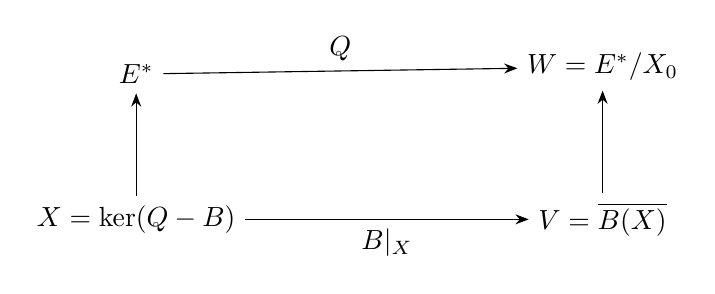
\begin{tikzpicture}[>=Stealth,node distance=13mm and 36mm]
\node (x) {$X=\ker(Q-B)$};
\node[right=of x] (v) {$V=\overline{B(X)}$};
\node[above=of x] (e) {$E^*$};
\node[above=of v] (w) {$W=E^*/X_0$};
\draw[->] (e) -- node[above] {$Q$} (w);
\draw[->] (x) -- node[below] {$B|_X$} (v);
\draw[->] (x) -- (e);
\draw[->] (v) -- (w);
\end{tikzpicture}
\caption{The new predual $X$. The square commutes because $Qx=Bx$ on
$X$, and $B(X)$ is dense in the closed span $V$ of the path cosets.
The vertical arrows are inclusions; restriction identifies $X^*$ with $E$.}
\label{fig:predual}
\end{figure}
\FloatBarrier


\begin{theorem}\label{twist:counterexample}
Under CH there is an infinite-dimensional real Banach space with no
separable infinite-dimensional quotient.
\end{theorem}

\begin{proof}
Use the space $X$ just constructed. Let $F\subset E$ be any
infinite-dimensional separable closed subspace, and put
\[
 C_F=\overline{\{y|_F:y\in X_0\}}\subset F^*.
\]
This space is separable. Indeed a countable dense subset of $F$ is
supported on a common countable set of coordinates; all other coordinate
functionals vanish on $F$. Since $X_0$ is the closed coordinate span,
its restrictions belong to the closed span of a countable family.

Restriction induces a bounded map
\[
 T_F:W\longrightarrow F^*/C_F,\qquad
 T_F(Qy)=y|_F+C_F.
\]
We claim that $T_F(V)$ is nonseparable. Otherwise its closure $M$ would
be separable. The inverse image of $M$ under the quotient map
$F^*\to F^*/C_F$ is then separable: its kernel $C_F$ is separable, and the restriction of the quotient map
to this inverse image still has the quotient norm.  More explicitly, lift
a countable dense set $(m_n)$ in $M$ to vectors $(u_n)$ in $F^*$, and
choose a countable dense set $(c_j)$ in $C_F$.  For any vector $z$ in the
inverse image, first make its quotient close to $m_n$.  The quotient norm
then makes $z-u_n$ close to a vector of $C_F$, which can in turn be
approximated by some $c_j$.  Thus the countable set
$\{u_n+c_j:n,j\ge1\}$ is dense in the inverse image.
But this inverse image contains every path restriction $P|_F$.
Theorem~\ref{branch:separation} supplies an uncountable norm-separated
family among those restrictions, a contradiction.

Because $\overline{B(X)}=V$, continuity gives
$\overline{T_F(BX)}=\overline{T_F(V)}$; hence $T_F(BX)$ is nonseparable.
For $x\in X$ we have $Qx=Bx$, so the evaluation image
$\{x|_F:x\in X\}\subset F^*$ has a nonseparable image in $F^*/C_F$.
It is itself nonseparable. Given any infinite-dimensional separable closed $F'\subset X^*$,
apply this conclusion to $F=R^{-1}(F')$.  Composition with the bounded
isomorphism $R|_F:F\to F'$ identifies the two evaluation images and
preserves norm separability.  Thus the evaluations on every such $F'$
are nonseparable. The necessary direction of Proposition~\ref{ev:criterion}
therefore rules out a separable infinite-dimensional quotient of $X$.
\end{proof}

The scalar-field transfer of Section~\ref{sec:fields} supplies a
complex counterexample as well. This is a consequence of the finite-sum
lemma there, rather than of the positive real-to-complex implication.

\begin{corollary}\label{twist:density}
Under CH, the real counterexample $X$ constructed above satisfies
$\dens X=\dens X^*=\aleph_1$. Its complexification is a counterexample
over $\C$ of norm density $\aleph_1$.
\end{corollary}

\begin{proof}
Lemma~\ref{ch:norm} makes the finitely supported rational vectors a
dense subset of $E$ of cardinality $\aleph_1$, while the coordinate
vectors $e_\alpha$, $\alpha<\omega_1$, are pairwise at distance at
least one. Hence $\dens E=\aleph_1$, and the isomorphism $E\simeq X^*$
from Lemma~\ref{twist:lemma} gives $\dens X^*=\aleph_1$.

Choose a norm-dense set $D\subset S_{X^*}$ of cardinality $\aleph_1$,
and, for each $f\in D$, choose $x_f\in S_X$ with $|f(x_f)|>1/2$.
The vectors $x_f$ have dense linear span: otherwise Hahn--Banach
supplies $g\in S_{X^*}$ vanishing on their closed span, and choosing
$f\in D$ with $\|f-g\|<1/2$ contradicts $|f(x_f)|>1/2$.
Rational linear combinations of these vectors give $\dens X\le\aleph_1$.
The space $X$ cannot be separable, since it is infinite dimensional
and would then be its own forbidden quotient. Thus $\dens X=\aleph_1$.

The complexification in Corollary~\ref{ev:fields} has underlying real
space isomorphic to $X\oplus_\infty X$, so it has the same density.
That corollary also gives the absence of separable infinite-dimensional
complex quotients.
\end{proof}

\section{Set-theoretic models and consistency bounds}\label{model:section}

The analytic implications concern Banach spaces inside a fixed model of
set theory.  We now verify that their hypotheses give the two required
relative-consistency statements.  Choice is retained throughout.

Real-valued measurability and its strict additivity convention are as defined
in the introduction; this agrees with \cite[Definition~1.1]{Caicedo2006}.
Atomlessness is a separate property and is not part of that definition.

We use the following preservation theorem of Solovay
\cite[Theorem~7]{Solovay1971}, in the formulation recorded in
\cite[Fact~1.27]{Caicedo2006}.

\begin{theorem}[Solovay]\label{model:solovay}
If $\kappa$ is real-valued measurable, then forcing with a measure algebra
preserves its real-valued measurability.  In particular, in the extension
there is a $\kappa$-additive probability measure on the full power set of
$\kappa$ in that extension, vanishing on singletons.
\end{theorem}

Here a measure algebra is the Boolean algebra of measurable sets modulo
null sets of a probability space, with zero omitted when it is used as a
forcing notion.  The special case of Theorem~\ref{model:solovay} used
below also has a direct proof in
\cite[Section~2, Lemmas~2.1--2.4]{FuchinoGreenbergShelah2006}.
That construction measures every subset of $\kappa$ in the extension,
is countably additive, and makes unions of fewer than $\kappa$ null sets
null. These properties give the stated additivity: in a disjoint family
of size less than $\kappa$, only countably many members have positive
measure, and the union of the remaining members is null.

\begin{proposition}\label{model:positive}
If ZFC with a measurable cardinal is consistent, then ZFC with a
real-valued measurable continuum is consistent.
\end{proposition}

\begin{proof}
Work in a ground model of ZFC with a measurable cardinal $\kappa$.
A $\kappa$-complete nonprincipal ultrafilter on $\kappa$ gives a
$\{0,1\}$-valued probability measure witnessing its real-valued
measurability.

We first record the cardinal arithmetic needed to control the continuum.
The cardinal $\kappa$ is regular: sets of size less than $\kappa$ are
null, so a cofinal union of fewer than $\kappa$ such sets cannot cover
$\kappa$.  It is also a strong limit.  Otherwise, for some
$\lambda<\kappa$ there would be an injection
$e:\kappa\to\mathcal P(\lambda)$.  For each $\xi<\lambda$, the ultrafilter
chooses one of the two sets on which the statement $\xi\in e(\alpha)$ is
constant.  Their intersection belongs to the ultrafilter by
$\kappa$-completeness, although injectivity makes that intersection have
at most one element.  This is impossible.  Every countable sequence of
ordinals below $\kappa$ is therefore bounded, and
\[
  \kappa^{\aleph_0}
   \leq \sum_{\lambda<\kappa}\lambda^{\aleph_0}
   \leq \kappa.
\]
Here $\lambda^{\aleph_0}\leq
2^{\max(\lambda,\aleph_0)}<\kappa$ for every $\lambda<\kappa$.
The reverse inequality is immediate, so
$\kappa^{\aleph_0}=\kappa$.

Let $\mathbb B_\kappa$ be the measure algebra of the fair-bit product on
$2^{\kappa\times\mathbb N}$.  We use the probability space generated by
finite-coordinate cylinders, or its completion; the quotient algebra is
the same.  Every element of this algebra has a representative determined
by countably many coordinates.  Such a representative is the inverse
image of a Borel set in a countable product.  Thus
\[
 |\mathbb B_\kappa|
 \leq \kappa^{\aleph_0}\,2^{\aleph_0}=\kappa
\]
in the ground model.  An antichain consists of disjoint nonzero elements
modulo null sets and hence is countable: for each positive integer $n$,
only finitely many of its elements can have measure greater than $1/n$.
Consequently the forcing has the countable chain condition and preserves
cardinals
\cite[Chapter~VII, Theorem~5.10]{Kunen1980}.

The generic coordinate sequences give $\kappa$ distinct reals.  Indeed,
for distinct $\alpha,\beta<\kappa$, the event that their coordinate
sequences agree has product measure zero. For the reverse bound, every real
has a name specified by countably many antichains deciding its bits.  Each antichain is countable, so at most
$|\mathbb B_\kappa|^{\aleph_0}\leq\kappa$ such deciding-antichain descriptions
suffice to name all reals
\cite[Chapter~VII, Definition~5.11 and Lemmas~5.12--5.13]{Kunen1980}.
Hence the extension satisfies $\mathfrak c=\kappa$.

Theorem~\ref{model:solovay} now gives the required measure on
$\mathcal P(\mathfrak c)$ in the extension.  Set forcing preserves ZFC,
including Choice~\cite[Chapter~VII, Theorem~4.2]{Kunen1980}.
The definable forcing relation and truth theorem
\cite[Chapter~VII, Theorems~3.5--3.6]{Kunen1980} give the asserted
relative-consistency implication in their syntactic, or finite-fragment,
interpretation~\cite[Chapter~VII, Sections~1 and~9]{Kunen1980}:
a finite contradiction proof in the extension theory would yield one in
the ground theory. This requires no transitive set model of all ZFC.
\end{proof}

\subsection*{Completion of the relative-consistency argument}
Let $\mathrm{SQ}_{\mathbb R}$ and $\mathrm{SQ}_{\mathbb C}$ denote the
separable quotient assertions over the indicated scalar fields.
Applying Theorem~\ref{pos:theorem} and Proposition~\ref{ev:positive-transfer} to
Proposition~\ref{model:positive} yields, for each
$\mathbb F\in\{\mathbb R,\mathbb C\}$,
\[
 \operatorname{Con}(\mathrm{ZFC}+\text{there is a measurable cardinal})
 \ \Longrightarrow\
 \operatorname{Con}(\mathrm{ZFC}+\mathrm{SQ}_{\mathbb F}).
\]
On the other side, G\"odel's constructible-universe theorem
\cite{Godel1938}, in the formulation of
\cite[Chapter~VI, Corollary~4.9]{Kunen1980}, gives
$\operatorname{Con}(\mathrm{ZFC})\Longrightarrow
\operatorname{Con}(\mathrm{ZFC}+\mathrm{CH})$.
Theorem~\ref{twist:counterexample}, together with Corollary~\ref{ev:fields},
therefore gives
\[
 \operatorname{Con}(\mathrm{ZFC})
 \ \Longrightarrow\
 \operatorname{Con}(\mathrm{ZFC}+\neg\mathrm{SQ}_{\mathbb F})
 \qquad(\mathbb F=\mathbb R,\mathbb C).
\]
Under the measurable-cardinal consistency hypothesis both sides are
consistent with ZFC.  Therefore ZFC proves neither
$\mathrm{SQ}_{\mathbb F}$ nor its negation, for either scalar field.

\subsection{Independence at density $\aleph_1$}

For the restricted assertion, the positive consistency bound can be
lowered using the earlier small-density theorem of Saxon and
S\'anchez Ruiz \cite{SaxonSanchezRuiz1996}: every infinite-dimensional
real Banach space of norm density less than $\mathfrak b$ has a separable
infinite-dimensional quotient; see \cite[Theorem~2.1]{Brech2025} for
its statement and a proof sketch. We explain the set-theoretic hypothesis that
makes this theorem apply at density $\aleph_1$.

The axiom $\mathrm{MA}_{\aleph_1}$ states that, in any nonempty partial order with
the countable chain condition, every collection of at most $\aleph_1$
dense sets is met by a filter. Full Martin's axiom, denoted by
$\mathrm{MA}$, requires this conclusion for every collection of fewer
than $\mathfrak c$ dense sets. The axiom $\mathrm{MA}_{\aleph_1}$ implies
$\mathfrak b>\aleph_1$.
To see this, fix a family $\mathcal A\subset\N^{\N}$ of cardinality at
most $\aleph_1$. A condition is a pair $(s,A)$, where $s$ is a finite
sequence of natural numbers and $A$ is a finite subset of $\mathcal A$.
A stronger condition $(t,B)$ extends $s$, contains $A$ in $B$, and
satisfies $t(n)\ge f(n)$ for every $f\in A$ and every new coordinate
$n$ of $t$. Conditions with a fixed stem $s$ have common extensions for
every finite subcollection: retain $s$ and take the union of their
finite sets. There are only countably many stems, so the partial order
is $\sigma$-centered and in particular has the countable chain condition.

For each $f\in\mathcal A$, the conditions with $f\in A$ form a dense
set. For each $n$, the conditions whose stem has length at least $n$
also form a dense set, since finitely many functions can be dominated
when a stem is extended. A filter meeting all these sets has a union
of stems $g\in\N^{\N}$. Once a condition has included $f$ in its finite
set, every common strengthening with a sufficiently long stem dominates
$f$ on the new coordinates. Directedness of the filter therefore gives
$f\leq^*g$. Thus $\mathcal A$ is bounded, proving
$\mathfrak b>\aleph_1$.

\begin{proof}[Proof of Corollary~\ref{intro:small-density}]
Starting with a ground model of ZFC and GCH, the forcing construction in
\cite[Chapter~VIII, Theorem~6.3]{Kunen1980} gives a model of Martin's
axiom with $\mathfrak c=\aleph_2$. G\"odel's constructible-universe theorem
and the relative-consistency interpretation of forcing therefore give
\[
 \operatorname{Con}(\mathrm{ZFC})\Longrightarrow
 \operatorname{Con}(\mathrm{ZFC}+\mathrm{MA}+\mathfrak c=\aleph_2).
\]
This model satisfies $\mathrm{MA}_{\aleph_1}$, hence
$\mathfrak b>\aleph_1$ by the preceding argument. The small-density
theorem gives a separable infinite-dimensional quotient for every real
Banach space of norm density $\aleph_1$. A complex Banach space has the
same norm density as its underlying real space, so
Proposition~\ref{ev:positive-transfer} gives the corresponding complex
conclusion.

On the other side, consistency of ZFC gives a CH model, and
Corollary~\ref{twist:density} supplies real and complex counterexamples
of norm density $\aleph_1$ there. Consequently, for each field
$\mathbb F\in\{\R,\C\}$,
\[
 \operatorname{Con}(\mathrm{ZFC})\Longrightarrow
 \begin{cases}
 \operatorname{Con}(\mathrm{ZFC}+\SQ^{\aleph_1}_{\mathbb F}),\\
 \operatorname{Con}(\mathrm{ZFC}+\neg\SQ^{\aleph_1}_{\mathbb F}).
 \end{cases}
\]
This proves the asserted independence with no large-cardinal consistency
hypothesis.
\end{proof}


\bibliographystyle{plain}
\bibliography{references}
\end{document}
